\chapter{Introducci'on}
% 
% Existen dos tipos de citas bibliograf'icas: usa \verb|\citep{..}| para
% citas en \emph{par'entesis} y \verb|\citet{..}| para citas
% en el \emph{texto}. Por ejemplo, estudios reciente han mostrado nuevos e
% interesantes modelos que se pueden aplicar para reformular teor'ias
% f'isicas~\citep{NewCam97}. Mientras que, el trabajo de \citet{Rofl06} fue
% considerado muy divertido por una significativa fracci'on de la comunidad
% de investigadores. Tambi'en es posible citar a varios trabajos en una sola
% referencia \citep{Lamport86,Knuth84}.

\section{Objetivos}


\section{Estructura de la tesis}

% La introduc Para poder  correctamente la aproximacion utilizada 
Este primer capítulo introductorio está dividida en dos secciones, que presentan los aspectos necesarios para comprender el trabajo realizado, el cual se centra en el diseño de nuevas secuencias linkers para el diseño de proteínas linkerss con 
propiedades estructurales y funcionales definidas, restringiendo las actividades biologicas y conformaciones no deseadas.
 
% En las secciones \ref{conformationalLandscape} y \ref{functionalLandscape} 
En la sección \ref{proteinLandscape} se intenta describir el amplio panorama conformacional y funcional que presentan las proteinas in-vivo, describiendo cuales son los posibles destinos de las proteinas desde que son sintetizadas en el ribosoma
Se desarrollan los conocimientos actuales acerce del perfil de conformaciones y funciones conocidas, y las propiedades secuenciales asociadas con estas.
Se intenta describir como estos conocimientos actuales sobre las propiedades conformacionales y funcionales de las proteinas se trasladan en el desarrollo 
de un amplio abanico de metodos y herramientas bioinformaticas que, a su vez, permiten nuevos avances en los conocimientos subyacentes.

En la sección \ref{proteinEngineering} se desarrolla el tema de ingenieria de proteínas, intentando mostrar los conceptos mas relevantes del área asociados a este trabajo, introduciendo el problema de la obtención/diseño de linkers artificiales.

En el capítulo \ref{method} se detalla el método implementado para obtener secuencias linker, indicando los fundamentos, limitaciones y aspectos relevantes de su utilización.

En el capítulo \ref{tools} se detalla el conjunto de herramientas utilizadas para evaluar propiedades estructurales y funcionales de interés, describiendo el objetivo de cada evaluación y . 

En el capítulo \ref{results} se muestran, en primer lugar, las evaluaciones realizadas para obtener los parámetros óptimos de ejecución. 
Además, se evaluan distintas propiedades de la herramienta resultante y su ejecución analizando, luego, las secuencias obtenidas. 


\section{Perfil conformacional y funcional de proteinas}
\label{proteinLandscape}

\subsection{Propiedades conformacionales de las proteinas}
\label{conformationalLandscape}

\begin{itemize}
 \item proteinas globulares, fibrosas y de membrana
 \item folding
 \item estados intermedios de plegamiento
 \item IDPs
 \item misfolding + aggregation + amyloid formation
\end{itemize}


% la idea de esta introduccion es describir conformational-functional landscape de las proteinas en la celula





% esta parte de estructuras individuales podria ir en 
The structure-function paradigm claims that a specific function of a protein is determined by its unique and rigid three-dimensional (3D) structure. 
Thus, following its biosynthesis on the ribosome, a protein must fold to a native, defined 3D structure to be functional. 
The primary origin of this structure-function paradigm is the “lock and key” hypothesis formulated in 1894 by Emil Fischer to explain the astonishing specificity of the enzymatic hydrolysis of glucoside multimers by different types
of similar enzymes. For a long period of time, the validity of “lock and key” model and its associated sequence-structure-function paradigm was unquestioned, especially after the crystal structures of proteins started to be solved by X-ray diffraction

Este paradigma se deriva de los primeros avances en el estudio de estructuras de proteinas. Over the past century evidence steadily accumulated that a well-defined structure is the prerequisite of protein function.

Basic biology and biochemistry textbooks that explain biological phenomena at the molecular level exquisitely rely on this notion, the ‘structure–function paradigm’.

The explanatory power of these 3-D
structures continued to reinforce the static view of protein

Throughout the 20th century, tens of
thousands of structures have been solved and deposited in the
Protein Data Bank (PDB), supporting again the necessity of a 3-
D structure for functionality.
structure that remained unquestioned.
In contrast to this view,
already in 1958 Koshland suggested the “induced-fit” model
based on the observations that some enzymes could act on
differently shaped substrates and hence a degree of flexibility is
inevitable in function. 2

A well-folded, albeit dynamic,
structure was thought to be the hallmark of protein function.



Although deviations from this norm were always apparent, they had been invariably neglected or ignored.
Mas adelante en el tiempo se fue encontrando que, además de las estructuras globulares funcionales mas estudiadas, proteins also populate various other states under native, functional conditions, including disordered and partially ordered conformations, and different aggregated assemblies.
Although it was evident from early studies that both soluble and fibrillar forms of proteins could exist (33 ????) , most attention was focused on the soluble states that were found to possess demonstrable biological function.


Furthermore, questions such as, “what does the missing
electron density in most of the deposited structures in the PDB
correspond to?”, “why are some proteins highly sensitive in vitro
to proteolysis?”, and “why do some proteins possess a particular
behavior during the purification process?” further opened eyes
toward flexibility and focused attention on proteins basically
distinct from well-known globular proteins. A combined answer
to these questions ruled out flexible proteins as artifacts and
enlightened the “dark side” of structural biology, that of
disordered proteins (i.e., proteins that lack 3-D structure).



Wright and Dyson 8 suggested that the existence of proteins with intrinsic protein disorder calls for a reassessment of the protein–structure– function paradigm.




En el grafico (*** poner grafico de proteostasis que tiene un estado 'nativo' , un estado 'misfolded' y los demas estados de agregacion, etc) se ve que al sintetizarse, 
la proteina naturalmente tiende a ir adquiriendo una conformacion estructural (conjunto de conformaciones mas restringida).
Lo que se fue desarrollando en los ultimos años es que el estado funcional no pertenece(siempre) a una estructura altamente definida sino que puede pertenecer a un conjunto de conformaciones que van desde
estado plegado hasta estados desestructurados, que pueden confundirse con estados totalmente desordenados. 
% fall onto a structural continuum, from tightly folded single domains, to multidomain proteins that might have flexible or disordered regions, to compact but disordered MOLTEN GLOBULES and, finally, to highly extended, heterogeneous unstructured states 
Thus, not just the ordered state but any of the known polypeptide conformations can be the native state of a protein.

Las sintesis de proteínas en el ribosoma puede verse mejor como el punto de inicio para que cada proteina tome una ruta particular a medida que emerge y se acopla al entorno celular. 
Entre las posibles rutas esta la adquisicion de un continuo de estructuras conformacionales funcionales, la adquisicion de una estructura distinta a la funcional(misfolding), y una variedad de estados de agregacion.

% adquiera un continuo de estructuras conformacionales funcionales a medida q emergen y se acoplan al entorno celular.% adoptando la estructura que la caracteriza .

Es por esto que las propiedades conformacionales de una proteína quedan mejor definidas si se declara el conjunto de multiples estados accesibles por sus estructuras.
% A este continuo de conformaciones que pueden adoptar las proteinas individuales, se agregan distintos tipos de estados agregados, conformados a partir de uniones entre proteinas en distintas conformaciones iniciales(conformaciones desestructuradas, intermedios o plegados).
De acuerdo con esta forma de ver, esta accesibilidad estará dada por la estabilidad termodinámica de cada conformacion accesible y la cinética de interconversión entre estas.
Estos requerimientos pueden indicar por ejemplo q ciertos estados altamente estables como puede ser las fibras amiloides no sean estados naturales comunes debido a los requerimientos cinéticos, a pesar de ser termodinamicamente estables.
% De acuerdo con esta forma de describir las posibles conformaciones de las proteinas, the various fates awaiting a polypeptide chain once it has been synthesized in the cell 
% will depend on the kinetics and thermodynamics of the various equilibria between di¡erent possible states.

Las propiedades cinéticas y termodinámicas están dadas por el contexto celular (pH, iones, concentracion de proteinas, presencia de otras moleculas con las que interactúa, etc) y, obviamente, por los posibles cambios que puede tener una proteina,
ya sean mutaciones o modificaciones postraduccionales.
% Las propiedades estructurales de una proteina, descritas de esta forma, pueden modificarse para una proteina a partir de cambios en el contexto(pH, iones, concentracion de proteinas, presencia de otras moleculas con las que interactúa, etc) 
% y, obviamente, también a partir de mutaciones o modificaciones quimicas sobre ésta. 
Esta forma de ver las propiedades estructurales permite ver los origenes de los cambios conformacionales desde el punto de vista de las propiedades fisicoquimicas de las proteinas.
If the stability or cooperativity of the native state of a protein is reduced, for example by a mutation, the population of non-native states will increase.


Es importante destacar, entonces que, for a given polypeptide chain a chosen fate is not a final one, and a choice may be further modulated by environmental pressure. 
Thus, intrinsically unstructured proteins may be forced to fold or misfold via modification of their environment (addition of natural binding partners, changes in properties of solvent and so on), whereas a destabilizing environment may push a natively
folded protein to the misfolding route. Alternatively, the
presence of chaperones may reverse the misfolding route
and effectively dissolve small aggregates




Durante la última década, uno de los mayores cambios en el campo de las proteínas ha sido el reconocimiento de la ubicuidad e importancia de las proteínas intrínsecamente desordenadas. 
% \cite(INTRINSICALLY UNSTRUCTURED PROTEINS AND THEIR FUNCTIONS)
Las proteinas en solucion fall onto a structural continuum, from tightly folded single domains, to multidomain proteins that might have flexible or disordered regions, to compact but disordered MOLTEN GLOBULES and, finally, to highly extended, heterogeneous unstructured states (FIG. 1) 
% This continuum has been interpreted in terms of a ‘PROTEIN TRINITY’ (ordered, molten globule and RANDOM COIL 20 ) or ‘PROTEIN QUARTET ’ 
As the main criterion of a native protein is its ability to perform a biological function, these partially or completely disordered proteins must be regarded as native entities.


% Si bien decimos aca que las proteinas pueden adquirir estructuras correspondientes un ensamble de estructuras accesibles , es posible hacer una clasificación entre proteinas que adoptan estructuras plegadas(con un estado nativo definido por un pequeño conjunto de estructuras) 
% y proteínas intrínsecamente desestructuradas (que adoptan estructuras correspondientes a un gran ensamble continuo de conformaciones). Luego se tratará las conformaciones agregadas de proteínas como una dimensión conformacional distinta.



% PARA PODER DESCRIBIR DE FORMA SIMPLE LAS PROPIEDADES CONFORMACIONALES SE PUEDE INTENTAR HACER UNA CLASIFICACION DE LAS FORMAS ESTRUCTURALES ADOPTADAS POR LAS PROTEINAS EN SOLUCION. 
% EN FORMA GENERAL SE PUEDEN CLASIFICAR EN:
% 	-CONFORMACION PLEGADA. Este estado nativo puede dividirse ademas en: native (ordered), molten globule, pre-molten globule, and coil-like.
% 	-DISORDERED STRUCTURE (ID): podria considerarse como un conjunto de estados entre los cuales se interconvierte a diferentes velocidades.
% 	-MISFOLDED, AGREGATION,AMYLOID, ETC: generalmente no tienen caracteristicas estructurales definidas, ....




\subsubsection{Proteinas globulares, fibrosas y de membrana}



Obviously, the consideration of a protein as a rigid crystal-like entity is an oversimplification, since even the most stable and well-folded proteins are dynamic systems that possess different degrees of conformational flexibility.
This is because of the simple fact that so-called conformational forces, that is, forces stabilizing the secondary structure of a protein and its tertiary fold, are weak and can be broken even at ambient temperatures due to thermal fluctuations

Furthermore, one should keep in mind that not all proteins structures which are deposited to PDB are structured throughout their entire lengths. Instead, many PDB proteins
have portions of their sequences missing from the determined structures (so-called regions of missing electron density) 7,8 due to the failure of the unobserved atom, side chain, residue, or region to scatter
X-rays coherently caused by their flexible or disordered nature. Such flexible/disordered regions are rather common in the PDB, since only about 3\% of
protein structures deposited in the PDB do not have such regions of missing electron density.

% Para intentar clasificar(discretizar)
% the conformational space of globular proteins involves four general conformations(random cloil, pre-molten globules,molten globules, native).

  
% En el caso de proteinas altamente estructuradas, la búsqueda de la estructura nativa no es un proceso trivial, y ha promovido la investigación de estructura de proteínas durante muchos años
% El proceso mediante el cual una proteína adquiere (rápidamente) 
% HACER UNA PEQUEÑA INTRODUCCION AL PROCESO DE PLEGAMIENTO, MUY BREVE
Dado que la idea de esta sección es poder describir los destinos que tendrán las proteinas al ser sintetizadas en la celula, 
no vamos a desarrollar el proceso de plegamiento(siendo que, ademas, es un tema muy complejo) y nos vamos a centrar en las estructuras finales que se pueden encontrar y, cuando sea necesario, en estados intermedios semiestables que sean relevantes.

The sequences of natural proteins have emerged through evolutionary processes such that their unique native states can be found very efficiently even in the complex environment inside a living cell.
Lo que se sabe es que...In order to achieve the native state encoded by the fold, the protein molecule has to find its way to this unique conformation rather than one of the countless alternatives. 
Contemplation of this problem gave rise to the 'Levinthal paradox'. 
In vivo, the beginning of the folding process is the nascent chain as it emerges from the ribosome. 
In vitro, folding begins from a fully formed polypeptide chain that has been unfolded, usually by addition of a chemical denaturant such as urea. 
In both cases the polypeptide chain is highly disordered before folding is initiated. 
In the extreme case, approximated rather well for many proteins in denaturants, the protein is said to be in a `random coil' state, where only local steric interactions constrain the conformations adopted by the molecule.



These intermediates are characterized by substantial secondary structure and little tertiary
structure; a collapsed conformation more compact than the unfolded state; exposed hydrophobic surfaces, 
which lead to binding of hydrophobic dyes
and a propensity to aggregate; 
and a heat capacity similar
to that of the unfolded state. 
The term compact intermediates
encompasses a broad range of conformations
and degrees of
folding and compactness.
compact intermediates have no single, unique conformation, but rather a whole plethora of structures that range from being very
similar to the native state to being substantially expanded and significantly unfolded. 
The properties of compact intermediates from different proteins, and in some cases from the same protein under different conditions, may be significantly different. 
Equilibrium compact intermediates may be good models for transient intermediates formed during folding

Sufficient numbers of different proteins forming stable-equilibrium, partially folded conformations have been observed that we can
make the generalization that all proteins, under the appropriate conditions, will form such species.


The intermediates in the folding process can be classified in
% PONER LOS DISTINTOS ESTADOS INTERMEDIOS





\subsubsection{Proteinas intrínsecamente desestructuradas}

Varios reviews en \cite{uversky2010understanding,dyson2005intrinsically}.

Inicialmente, these proteins were independently discovered one-by-one over a long period of time and therefore they were considered as rare exceptions to the general rule.

The suggestion that the native state of many proteins is intrinsically disordered (or, as originally termed, unstructured) is now integral to our general view of protein structure and function.
Como se dijo en la introduccion, a little more than 10 years ago,however, such challenge to the almost dogmatic ‘structure–function paradigm’ was pure heresy due to the overwhelming evidence that structure determines function.
As it is often the case for new scientific concepts, the idea of structure-less functionality went through the stages of passive ignorance and active denial to scrupulous examination and enthusiastic acceptance
A decade of steady progress turned skepticism around.
Como parte de estos avances, en los ultimos años se han encontrado gran cantidad de proteinas que adoptan estructuras cuyas conformaciones son total o parcialmente desordenadas(segmentos globulares), soportando esta definicion, formalizada a principios de milenio. 
the transition in paradigm was enforced by scattered experimental observations of disorder in a few dozen proteins. 
% una de las dudas que se tenia era si este estado conformacional existia solo in vitro y en realidad in-vivo lo que ocurria era que el crowding generaba el plegamiento
Evidence added to that obtained by other techniques [mostly NMR and circular dichroism (CD)]..... and the evidence seems overwhelming now that structural disorder also exists in vivo and it is truly the native, functional state of these proteins.

En terminos energeticos, for an IDP, the energy landscape is characterized by the lack of a global minimum and by the presence of multiple local minima separated by low energy barriers. 
As a consequence, such a protein exists as a dynamic ensemble of interconverting structures, which can be described by relatively flat energy landscapes.
Estas secuencias presentan en solución un conjunto heterogéneo de conformaciones fácilmente maleable por cambios en el medio. 
Conditions, post-translational modifications,
and binding events (see section 6) change the relative free
energies of individual conformations as well as the energy
differences between conformations.
As a result, the
populations of individual conformations within the ensemble
change under different conditions. These individual states are
often important for function. Thus, the dynamic nature of IDPs is
best modeled by statistical approaches that describe the
probabilities of individual conformations in the ensem-
ble, 172,177,178 and is best measured by experimental techniques
that prevent conformational averaging.

En lugar del análisis estructural clásico basado en dominios globulares, podemos describir estos conjuntos conformacionales en términos de los promedios y desviaciones estándar de la distancia entre los extremos de la secuencia, el radio hidrodinámico, el contenido en estructura secundaria y otros parámetros (20).

Functional complexes of IDPs with their partners are formed via the specific intermolecular interactions that change the energy landscape creating more defined free energy minima.(ESTO LO PODRIA PONER EN LA PARTE DE INDUCED FIT)
A similar mechanism underlies the formation of the non-productive protein complexes (oligomers, amorphous aggregates, amyloid-like fibrils, etc.). Here, interactions of the disordered parts of IDPs or interactions of the denatured proteins result in the appearance of profound free energy minima.





% PROPIEDADES ESTRUCTURALES
A combination of experimental and theoretical studies has clarified how given sequences define specific free energy surfaces that enable folding.
A diferencia de estas superficies energeticas, caracteristicas de las estructuras con plegamiento definido, in some cases the native state of a given peptide or protein may not be structured in a globular form but disordered.
% ESTA LINEA PODRIA IR EN LA PARTE DE HOMEOSTASIS DE PROTEINAS
Regardless of its nature, however, the functional native state is likely to only reflect a local free energy minimum at physiological concentrations, as self-association into aggregated protein spe-
cies may in many cases lower the global free energy 41,42(BOX 1) . Indeed, the maintenance of protein solubility has emerged as a central aspect of the more general topic of protein homeostasis 3,43,44 .

Pero acá estamos hablando de un numero considerable de proteinas cuya secuencia encodes for the intrinsically unstructured proteins without specific structure.
These raise several compelling biophysical questions related to the structural characteristics of natively unfolded proteins. How unfolded are these proteins? Are they random coils, or do
they possess residual structure? If they have residual structure, how should they be classified?
Based on the analysis of the available literature, it has been concluded that intrinsically unstructured proteins do not possess uniform structural properties, as expected for members of a single thermodynamic entity.


In general, proteins with intrinsically disordered sequences cannot bury sufficient hydrophobic core to fold spontaneously into the highly organized 3D structures that characterize the proteins that are represented in the Protein Data Bank (see the online links
box). In some cases, compact but disordered molten-globule-like states can be formed, or local regions of the sequence can have a propensity to adopt isolated and fluctuating elements of secondary structure (which is equivalent to the ‘pre-molten globule’ proposed by Uversky 2 ). 

Structural disorder can now be studied in great detail by several dozen experimental techniques [21], and the most spectacular advance has been achieved through the application of multidimensional NMR. This approach is often
complemented by other structural techniques, such as small-angle X-ray scattering (SAXS), which is combined with advanced computational data integration based upon molecular dynamics (MD) simulations (Figure 1). These new
approaches [22] enabled the characterization of the full structural ensemble of several dozen IDPs

It is probable that proteins rarely, if ever, behave as true random coils, especially in non-denaturing media: even in their most highly unfolded states, proteins show a propensity to form local elements of secondary structure or hydrophobic clusters
Accumulated data nonambiguously show that they most likely represent the polymer coils below a critical point, even under harsh denaturing conditions.




En base a estas propiedades estructurales y el induced fit, en el review \cite{dunker2001intrinsically} se plantea una clasificacion del desorden en dos categorias: intermittent and constant.
The former describes protein molecular recognition domains and other regions that undergo order/disorder transitions to carry out binding or other functions. The latter describes regions such as
proteinaceous detergents, flexible linkers, entropic springs, entropic clocks and entropic bristles that remain disordered while carrying out function.

Two unexpected and important concepts have also emerged in the binding-folding paradigm. One is the intriguing observation that two IDPs/IDRs can bind each other in a process of mutual (synergistic) folding [47].
The other, even more confounding finding, is that recognition can proceed even in the lack of folding in the bound state. 
The many examples of such ‘fuzzy’ interactions demand the extension of the concept of structural disorder to the bound state.



Structurally, IDPs range from completely unstructured polypeptides (native coils, that resemble the highly unfolded states of globular proteins) to extended partially structured forms (native pre-molten globules) or even to compact disordered ensembles that may contain significant secondary structure (native molten globules)
ID proteins have dynamic structures that interconvert on a number of timescales and have been shown to have many similarities to non-native states of “normal” globular proteins, which(como se describio antes) may exist in at least four different conformations: native (ordered), molten globule, pre-molten globule, and coil-like.

a typi-
cal IDP/IDPR contains a multitude of elements cod-
ing for potentially foldable, partially foldable,
differently foldable, or not foldable at all protein seg-
ments. 68 As a result, different parts of a molecule
are ordered (or disordered) to a different degree.
This distribution is constantly changing in time
where a given segment of a protein molecule has dif-
ferent structures at different time points. As a
result, at any given moment, an IDP has a structure
which is different from a structure viewed at
another moment

However, already in some early studies, it was indicated that IDPs/IDRs could be crudely grouped into two major structural classes, proteins with compact and extended disorder, indicat-
ing that functional IDPs can be less or more compact
and possess smaller or larger amount of flexible sec-
ondary/tertiary structure.
Para dejar las cosas un poco mas claras vamos a intentar realizar una clasificacion de las ID proteins en terminos estructurales.
Usando esta analogia(similitud) con los estados intermedios del plegamiento, en \cite{uversky2010understanding} it has been established that ID proteins and regions under physiological conditions in vitro might 
contain collapsed-disorder (i.e., where ID is present in a form of molten globules) and extended-disorder (i.e., regions where ID is present in a form of random coil or pre-molten globule)

\begin{itemize}
 \item[Collapsed disorder: ] The structural properties of the molten globule (which was originally described as universal folding intermediate of globular proteins) are well known and
have been systematized in number of reviews. The protein molecule in this intermediate state has no (or has only a trace of) rigid cooperatively melted tertiary structure. However, it is characterized not only by the well-developed secondary structure, but also by the presence of some topology, i.e., relatively fixed mutual positioning of the secondary structure elements. A considerable increase in the accessibility of a protein molecule to proteases was noted as a specific property of the molten globule.
The transformation into this intermediate state is accompanied by a considerable increase in the affinity of a protein molecule to the hydrophobic fluorescence probes

 \item[Extended disorder: ] A significant number of sequences encodes for the extendedly disordered proteins that are characterized by low sequence complexity. Are these proteins
random coils, or do they possess residual or transient structure? If they have residual or transient structure, how should they be classified? Based on the analysis of the available literature, it has been concluded that such proteins do not possess uniform structural properties, as expected for members of a single thermodynamic entity.
In fact, they may be divided into two structurally different groups, intrinsic coils and intrinsic pre-molten globules, tal como se realiza en \cite{uversky2002natively}: 
 Proteins from the first group have hydrodynamic dimensions typical of considerably unfolded polypeptide chain in poor solvent (see below and fig. 1), and do not possess any (or almost any) ordered secondary structure. 
Proteins from the second group are more compact (see below and fig. 1), and exhibit some amount of residual secondary structure. However, they are still less dense than native globular or molten globule proteins
\end{itemize}



% ESTA CLASIFICACION DE LAS IDPs EN 2 ES LO QUE DA ORIGEN A LA TEORIA DE PROTEIN TRINITY, QUE DICE QUE:
% Native proteins should be conceptualized as part of the “protein trinity”
% They exist in one of three states—ordered, collapsed-disordered, extended-disordered. And protein function derives from any one of these three states founding member of a new protein class or from transitions between them.

This model was subsequently expanded to include the premolten globule (PMG) state, which corresponds to an intermediate state between the RC and the MG

El modelo resultante actual esta compuesto de 4 estados\ref{proteinQuartet} que indican los posibles estados nativos(funcionales) de las proteinas.



\begin{figure}[htbp]
\centering
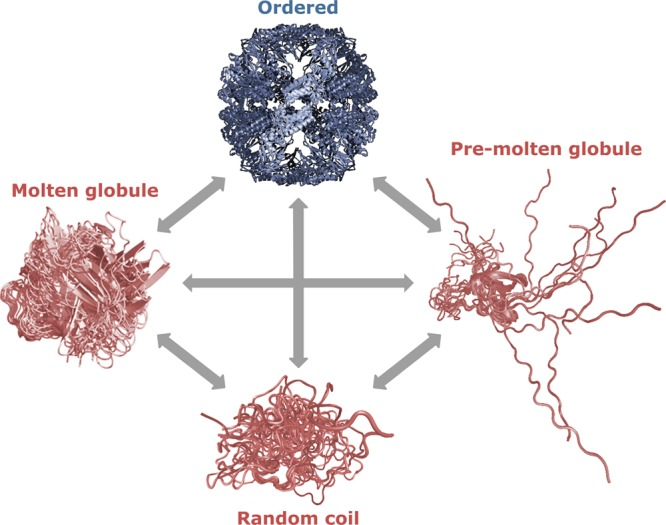
\includegraphics[width=0.7\textwidth]{img/proteinQuartet.jpg} 
\caption{Protein quartet model of protein function. Function can arise
from four different conformations of the polypeptide chain, or from
transitions between any of the states. \cite{uversky2002natively}}
\label{proteinQuartet}
\end{figure}





Due to their heteropolymeric nature, proteins are never random coils and always have some residual structure.
In fact, the existence of significant residual structure in the unfolded globular protein has been described even under the most
severe denaturing conditions, such as high concentrations of strong denaturants [144-147]. Thus, coil-like ID proteins are not completely random, but are characterized by the presence
of some residual (and highly flexible) structure. This fact is very important for the functioning of these proteins.
Protein random coils differ from true random coils in important respects, such as a non-random population of internal bond angles along the chain.
Thus, based on the exceptional structural heterogeneity of IDPs/IDPRs, IDPs are definitely much more structurally complex than random coil-like polypeptides.
Although this structural heterogeneity is very important for protein functionality, it represents a crucial hurdle for structural characterization of IDPs

Coincidiendo con esta idea que la proteina no plegada nunca es una true random-coil, the persistence of native-like contacts in the denatured (disordered) state has been shown in NMR experiements and in high temperature molecular dynamics simulation. The existence of preferred limited proteolysis cutting sites also indicates that the native conformation prevails

These and many other studies made the term unstructured obsolete. 
The distinguishing and unifying feature of these proteins,if any, is their inability to fold into a unique and stable tertiary structure.
They display a vast array of function-related structural organization, therefore, the field has settled on the term ‘disordered’. 
This term applies to both short and long regions that are part of a larger folded protein (loops and linkers) and proteins that entirely lack a folded structure. 
This latter category is sometimes also termed (natively) unfolded. 

many proteins are hybrids of ordered and disordered domains and regions, and this mosaic structural organization is crucial for their functions.



%  INDUCED FIT:
Although disordered proteins exist as dynamic structural ensembles without fixed tertiary structures, there is evidence that many flexible regions of proteins undergo coupled binding and folding \cite{dyson2005intrinsically}. 
A large decrease in conformation entropy accompanies such disorder-to-order transitions. 
An important feature of the intrinsically unstructured proteins is that they are able to undergo a disorder-to-or-der transition (i. e. partial or complete folding) during or prior to their biological function. 
In other words, intrinsically unfolded proteins in vivo are likely to be stabilized by functional binding to specific targets and ligands (such as a variety of small molecules, substrates, cofactors, other proteins, nucleic acids, membranes and so on). 
% Many intrinsically disordered proteins undergo transitions to more ordered states or fold into stable secondary or tertiary structures on binding to their targets — that is, they undergo coupled folding and binding processes.



IDPs fold as a whole while interacting with their partners, if the free energy of complex is lower than the free energies of IDP and its partner before their interaction.
More often, however, only a part of an IDP, a specific recognition element, which is a relatively short amphipathic linear motif contained within long disordered sequence, is involved in the coupled folding and binding events
Induced fit interactions can also occur between structural domains and relatively large natively unstructured regions of other proteins. 
The natively unstructured region is then induced to form a stable structure, but only in the presence of the interacting structural domain.

This disorder-to-order transitions, in turn, leads to a combination of high specificity and weak affinity, a pair of linked features that are extremely useful for signalling and regulation.

An often-raised issue with respect to IDP binding is whether folding occurs before or after binding (termed conformational selection and induced folding, respectively).
Detailed studies suggest that folding can occur both before and after binding in distinct cases


There are two major models describing the coupled folding and binding process in proteins, the conformational selection model and the simultaneous binding and folding model, also known as the induced folding model.

The conformational selection mechanism is based on the hypothesis that when free in solution, IDP populates the ensemble of conformations and, from this ensemble, the binding partner “chooses” or
“selects” a specific conformation which closely approximates that of the bound form. An illustrative example of the conformational selection mechanism in the recognition process is
so-called “preformed structural elements” or elements of local residual structure, which are frequently observed in IDPs and which are crucial for the IDP interactions with its specific
partners

Induced folding model postulates that IDP associates with its binding partner in a fully disordered state and subsequently folds in association with the target protein. 
In molecular recognition, this model is exemplified by so-called molecular recognition elements or features, which are short (around 20 residues) structural elements which are found 
within the regions of disorder and which mediates certain classes of binding
events of disordered regions undergoing a disorder-to-order transition into a specific structure that is stabilized by binding to its partner.
These recognition motifs can fold into $\alpha$-helix, $\beta$-strand, or form irregular structure on binding to a target protein

Obviously, in reality, either one of the outlined above mechanisms, the conformational selection model or the induced folding model, or some combination of the two can be used


En relacion a este concepto, nuevos conceptos han nacido para describir este tipo de entidades biologicas, en \cite{oldfield2005coupled} se 
Molecular Recognition Features (MoRFs) are short, interaction-prone segments of protein disorder that undergo disorder-to-order transitions upon specific binding, 
representing a specific class of intrinsically disordered regions that exhibit molecular recognition and binding functions.
Occupy a unique structural and functional niche in which function is a direct consequence of intrinsic disorder.

Different concepts regarding short recognition elements have been extensively discussed in the literature. Indeed, depending on whether the idea is approached from a structural point of view
or defined at the sequence level, a short motif could be denoted as a 'molecular recognition element' (MoRE)/'molecular recognition feature' (MoRF) or 'linear motif' (LM),
Moreover, Fuxreiter et al. in 2004 elaborated the concept of
preformed structural elements (PSEs) correlating the probable
structural preferences of IDPs in the unbound state

Molecular recognition by short recognition elements (motifs)
can be -and has been historically- approached from the
completely different direction of short sequence patterns
determining functional interactions and enzymatic modification,
i.e., LMs, ELMs, and SLiMs. 190,199,200 These motifs are linear in
the sense that 3-D organization is not required to bring distant
segments of the molecule together to build up the recognizable
unit.
The MoRF model describes regions
of intrinsic disorder that undergo a disorder-to-order
transition upon partner recognition, where the
residues responsible for these interactions are typi-
cally linear in the protein sequence.

En \cite{mohan2006analysis,vacic2007characterization} se hacen analisis mas extensos de MoRFs extraidos de PDB.
En estos analisis se intentan encontrar differences in residue composition and several geometric and physicochemical properties that can be used to discriminate MoRFs, with a high degree of accuracy


Disorder prediction of LMs and their flanking regions for
the experimentally characterized examples of the ELM database
(a database gathering eukaryotic linear motifs) (http://elm.eu.
org) 199 suggests that LMs and their flanking regions are segments
of intrinsic disorder within a more ordered environment



% ****************************
% ACA SE UNEN LOS CONCEPTOS DE PSEs, LMs, MoREs)  , ESTO LO PUEDO PONER AL FINAL CUANDO HABLO DE LINEAR MOTIFS EN LA PARTE DE FUNCIONALIDAD EN IDPs 
% *****************************
Although not fully substantiated, 201 the three concepts of short
recognition motifs (PSEs, LMs, MoREs) can probably be
considered as manifestations of the same underlying principle of
binding of an ordered partner by a short segment within a
disordered region, which undergoes a disorder-to-order
transition or induced folding upon binding.
They possess an
amino acid composition that resembles that of IDPs with some
notable deviations (i.e., specificity-determinant residues favoring
order) and they can even in some cases be already preformed in
the free state (PSEs, PreSMos)

En \cite{fuxreiter2007local} se concluye algo similar a esto.
The question addressed in
this paper is the relationship and the range of possible
correspondence between LMs and molecular recognition
elements in IUPs.
The results establish a
connection between LMs and molecular recognition elements of
intrinsically unstructured proteins (IUPs), which realize a non-
conventional mode of partner binding mostly in regulatory functions.

results suggest that LMs and molecular recognition
elements of IUPs significantly overlap, and in the majority of
cases represent an equivalent set of motifs in modular proteins.

The molecular mode of action of
LMs and recognition elements of IUPs overlap, and probably
reflect a similar phenomenon viewed from different angles thus
far.
Whereas LMs have been identified as short sequence motifs
critical in recognition functions, primary contact sites (Csizmok
et al., 2005), preformed structural elements (Fuxreiter et al.,
2004) and molecular recognition elments/features (Mohan
et al., 2006; Oldfield et al., 2005) have been approached from
the direction of protein disorder, emphasizing recognition
segments embedded in such regions. Unity of these concepts
is underlined by the key role of a few specificity determinants in
all these recognition elements, and also by their local
preferences for undergoing disorder-to-order transition upon
molecular recognition (Dyson et al., 2002), which might already
be manifested prior to binding (Fuxreiter et al., 2004). Apart
from a minority of the cases when LMs are constituted of
segments of ordered domains, these different concepts of short
recognition elements express the same underlying physical and
functional principles that provide a probably widespread
solution to the dynamic control of protein-protein interaction
networks (data not shown).




% puedo extender el tema aca o derivarlo a la parte de funcionalidades

%******** UN POCO MAS EN DETALLE (COPIADO DE UN REVIEW DE 2011)
% The key characteristics of a MoRF are
% that it is the site of binding of the disordered protein to a partner, and that it undergoes some
% form of disorder-to-order transition upon binding. MoRFs were classified as α-MoRFs, β-
% MoRFs and ι(iota)-MoRFs, according to whether α-, β-, or irregular secondary structure type
% was formed upon binding (it is not clear how to classify a sequence such as Hif-1α, which
% forms α-structure in one complex (Freedman et al., 2002; Dames et al., 2002a) and β-
% structure in another (Elkins et al., 2003; Lee et al., 2003)). MoRFs may have a propensity for
% formation of residual structure in the free state (Mohan et al., 2006; Kim et al., 2009)
% although this may be hard to detect experimentally (Zor et al., 2002). At least in the case of
% the short linear motifs recognized by SH2, SH3 and Ser/Thr kinase domains, these
% sequences may be conserved between species (Ren et al., 2008)

% The past few years have
% seen a meteoric increase in the number and richness of the systems where coupled folding
% and binding are seen. This field has been reviewed several times recently (Dyson and
% Wright, 2002; Dyson and Wright, 2005; Wright and Dyson, 2009; Uversky, 2010), this
% concept is central to the entire rationale for the existence of IDPs that work on several
% systems.
% A recent rather comprehensive compendium of disorder-related complexes can
% be found in (Uversky, 2010).


Ten years ago, only predictor of natural disordered regions (PONDR) was available [14]; today, one can use any of about 50 predictors, which are based on several different principles \cite{he2009predicting}.
Como parte de estos ultimos años de investigacion se encontro una gran cantidad de funcionalidades y mecanismos asociados a proteins IDP(ver seccion funciones).
Se desarrollaron tambien bases de datos específicas \cite{sickmeier2007disprot,fukuchi2012ideal}, y aplicaciones bioinformáticas capaces de identificar el desorden intrínseco (19).
Intriguingly, thousands of the structures in PDB are now known to contain disordered chains that become structured only in the presence of the partner, and there are also many regions that are actually missing from electron density maps

% The identification of many IDPs  enabled the development of sophisticated bioinformatic algorithms for predicting disorder from sequence, which further advanced the field.
The availability of such predictors further advanced the field.
Based on predictions, we know that structural disorder is abundant in all species, and due to its strong correlation with regulatory and signaling functions, its level is significantly higher in eukaryotes than in prokaryotes
Although it has become almost commonplace in the field that structural disorder increases with the complexity of the organism, the highest levels are not witnessed in the most complex metazoan eukaryotes (e.g., in humans), but in single-celled eukar-
yotes that lead a host-changing lifestyle

% TERMINOLOGIA
En un principio se comenzo a definir a este tipo de secuencias como desestructuradas, indicando que prescindian completamente de estructura, aun sabiendo que they have potentially function-related
short- and long-range structural organization, which eventually called upon a change in terminology.
At that time, high-resolution data were rather limited, thus the concept was mostly phrased from the global structural level, which suggested that IDPs fall into coil-like, pre-molten globuletype and molten-globule types
% aca deberia ir algo sobre estudios estructurales que se han hecho
These and many other studies made the term unstructured obsolete. 
% IMPORTANTE
The distinguishing and unifying feature of these proteins – if any – is their inability to fold into a unique and stable tertiary structure
The terms intrinsically unstructured and natively unfolded may be also be suitable for extended random coils and even those that are collapsed, but these terms don't seem to appropriately describe proteins that form transient or
stable secondary structure. The term disorder suffers because of its negative connotation and its possible confusion with a pathological state, yet, on the other hand, disorder can be used for proteins like the molten globule that form substantial secondary structure but that
nevertheless are highly dynamic and non-uniform. For this last reason, herein we will call these proteins “intrinsically disordered” (ID).
By “intrinsic disorder” we mean that the protein exists as a structural ensemble, either at the secondary or at the tertiary level.

% DISORDER vs FLEXIBILITY:
Disorder and flexibility are often used synonymously, but the two terms are quite distinct\cite{radivojac2004protein}. With regard to an ordered protein, flexibility refers to the magnitudes of the excursions of the atoms from their equilibrium positions.
For a disordered region, variation in flexibility refers to differences in the speed of interconversion among the various members of the structural ensemble. 
A variety of methods have been used to investigate the flexibilities of disordered regions and proteins, including NMR.

Control of structural flexibility is essential for the proper functioning of a large number of proteins and multiprotein complexes. 
At the residue level, such flexibility occurs due to local relaxation of peptide bond angles whose cumulative effect may result in large changes in the secondary, tertiary or quaternary structures of protein molecules. 
Such flexibility, and its absence, most often depends on the nature of interdomain linkages formed by oligopeptides.

Analyses of structures(por ej. mediante X.ray diffraction) have shown that protein motion may occur due to conformational changes in individual residues or at the secondary, tertiary, or quaternary structural levels. Lactate dehydrogenase, triose-phosphate isomerase, as well as hemoglobin and related proteins are some of the earliest examples of proteins that showed conformational changes with important functional implications.







% COMPOSICION
Identification of IDPs as unique entities belonging to a new protein tribe is directly related to the recognition that their amino acid sequences are dramatically different from those of ordered proteins.
En otras palabras, since amino acid sequence determines three-dimensional structure, amino acid sequence should also determine lack of three-dimensional structure.


the absence of regular structure in these proteins has been explained by the specific features of their amino acid sequences including the presence of numerous uncompensated charged groups (often negative); 
 i.e., a high net charge at neutral pH, arising from the extreme pI values in such proteins , and a low content of hydrophobic amino acid residues.
Several ID proteins have been discovered due their unusual amino acid sequence compositions

It has been concluded that the combination of low mean hydrophobicity and relatively high net charge represents an important prerequisite for the absence of compact structure in proteins under physiological conditions. This observation was used to develop a charge-hydropathy (CH) plot method of analysis that distinguishes ordered and disordered proteins based only on their net charges and hydropathies.
From the physical viewpoint, such a combination of low hydrophobicity with high net charge as a prerequisite for intrinsic unfoldedness makes perfect sense: high net charge leads to charge-
charge repulsion, and low hydrophobicity means less driving force for protein compaction. In other words, these features are characteristic for ID proteins with the coil-like (or close to coil-
like) structures.
The disordered proteins are significantly depleted in bulky hydrophobic (Ile, Leu, and Val) and aromatic amino acid residues (Trp, Tyr, and Phe), which would normally form the hydrophobic core of a folded globular protein, and also possess low content of Cys and Asn residues.
The depletion of ID protein in Cys is also crucial as this amino acid residue is known to have a significant contribution to the protein conformation stability via the disulfide bond formation or being involved in coordination of different prosthetic groups.
On the other hand, ID proteins were shown to be substantially enriched in polar, disorder-promoting, amino acids: Ala, Arg, Gly, Gln, Ser, Glu, and Lys and also in the hydrophobic, but structure braking Pro.

The fact that natively unfolded proteins, with their depleted hydrophobicity, are noncompact under physiological conditions indicates that ‘salted water’ (typical ‘physiological’ buffer contains 100–150 mM NaCl) does not represent for them a poor solvent.
In other words, these
conditions do not force polymer segments to interact
specifically with each other and, thus, do not force them
to be effectively excluded from the solvent. On the other
hand, it has already been noted that even high concentra-
tions of strong denaturants do not represent a good sol-
vent for a polypeptide chain encoding for a typical glob-
ular protein, and a globular protein was assumed to never
be a random coil.


The fact that the sequences of ordered and disordered proteins and regions are noticeably different suggested that IDPs clearly constitute a separate entity inside the protein kingdom, 
that these proteins can be reliably predicted using various computational tools, 37–42 and structurally, 
that IDPs should be very different from ordered globular proteins since peculiarities of amino acid sequence determine protein structure.

Por lo tanto, a signature of probable intrinsic disorder is the presence of low sequence complexity and amino-acid compositional bias, with a low content of bulky hydrophobic aminoacids (Val, Leu, Ile, Met, Phe, Trp and Tyr), which would
normally form the core of a folded globular protein, and a high proportion of particular polar and charged amino.....ESTAS PROPIEDADES SE HAN UTILIZADO PARA LAS PRIMERAS GENERACIONES DE HERRAMIENTAS PARA PREDECIR DESORDEN A PARTIR DE LA SECUENCIA.
Luego se crearon predictores que analizaban la secuencia usando ventanas(PONDR)

In addition to amino-acid composition, the disordered segments have also been compared with the ordered ones by various attributes such as hydropathy, net charge, flexibility index, helix
propensities, strand propensities, and compositions for groups of amino acids such as W + Y + F (aromaticity).

Estas propiedades fisicoquimicas tambien fueron incluidas para los predictores.




% COMPLEJIDAD DE LAS IDPs
It was pointed out that IDPs possess noticeable
amino acid biases, and many IDPs/IDPRs are char-
acterized by sequence redundancy and low sequence
complexity, containing long stretches of various
repeats and being completely devoid of some (often
many) types of amino acid residues. These observa-
tions seem to indicate that the sequence space of
IDPs/IDPRs should be simpler than that of ordered
proteins.
However, the reality is more complex than
conventional wisdom might suggest, and the
sequence space attainable by simple IDPs/IDPRs is
more diversified than that of the structurally more
sophisticated ordered proteins.
In fact, a 100 resi-
due-long protein in which any of the normally occur-
ring 20 amino acids can be found has a sequence
space of 20 100 (10 130 ) sequences. 54 Obviously, not
all random amino acid sequences can fold into
unique structures. In other words, a sequence space
of a foldable protein (or “foldable” sequence space) is
noticeably smaller than the entire sequence space
available for a random polypeptide chain.

foldable proteins fold first and
then bind to their partners whereas IDPs/IDPRs
remain disordered until they interact with their
partners. 68,69 Furthermore, many IDPs/IDPRs do
not require folding to be functional, 1,4,13,14,70–73 and
some of them form fuzzy complexes, in which they
preserve significant amount of disorder. 74,75 All this
suggests that the sequence space of IDPs (at least
those which either do not fold at all or do not com-
pletely fold at binding) is noticeably greater than
the “foldable” sequence space due to the removal of
restrictions posed by the need to gain ordered struc-
ture spontaneously. 68 This represents one of the
conundrums of intrinsic disorder, where the appa-
rent sequence redundancy and simplicity are com-
bined with the lack of structural restrains leading to
the increase in the dimensions and complexity of the
available sequence space.



% ANATOMIA MODULAR DE LAS IDPs ******** ESTO PUEDE IR EN LA PARTE DE FUNCIONALIDAD DE IDPs PARA INTRODUCIR EL CONCEPTO DE SLMs

Since the unique 3D-structure of an ordered
single-domain protein is defined by the interplay
between all (or almost all) of its residues, one could
expect that the structure-coding potential is homoge-
neously distributed within its amino acid sequence.
On the other hand, a sequence of an IDP/IDPR con-
tains multiple, relatively short functional elements
and therefore represents a very complex structural
and functional mosaic. 68 This important feature
defines the known ability of an IDP/IDPR to inter-
act, regulate, and be controlled by multiple structur-
ally unrelated partners. 76 Such functional “anatomy”
of IDPs/IDPRs is determined by the extremely high
level of their sequence heterogeneity, which is fur-
ther increased due to the ability of a single IDPR to
bind to multiple partners gaining very different
structures in the bound state. 77




Todas estas propiedades hacen que parezca razonable que este tipo de proteínas este altamente regulada dentro de la célula \cite{gsponer2008tight}.

It is clear now that the IDPs and IDPRs are real, abundant, diversified, and vital. The highly dynamic nature of IDPs and IDPRs is a visual illustration of the chaos.
the evolutionary persistence of these highly dynamic proteins (see below), their unique functionality, and involvement in all the
major cellular processes evidence that this chaos is tightly controlled



Cada tipo de macromolécula está compuesta por una clase distinta de monómeros. En el caso

\subsubsection{Misfolding \& Aggregation}

As has been already noted, the sequences of proteins have
evolved in such a way that their unique native states can
be found very efficiently even in the complex environ-
ment inside a living cell.

However, under some condi-
tions, proteins fail to fold properly or to remain correctly
folded; this misfolding can lead to the development of
different pathological conditions.

contrary to the process of productive protein folding, leading to the appearance of rigid conformation with specific function, the end products of misfolding may have a different appearance. 
The morphology of these end products depends on the particular experimental conditions, and misfolded product may appear as soluble oligomers, amorphous aggregates or amyloid-like fibrils. 
Any of these three species could be cytotoxic, thus giving rise to the development of pathological conditions. 
The reason for such a morphological difference is potentially connected with the diversity of the partially folded intermediates favoring protein self-association. 
In fact, multiple environmental factors, such as point mutations, decrease in pH, increase in temperature, the presence of small organic molecules or metal ions, and other charged molecules, might induce structural rearrangements within a protein molecule, shifting equilirium toward the partially folded conformation(s). As different factors may stabilize slightly different partially folded intermediates, the formation of morphologically
different aggregates is expected.


Como se dijo en las secciones cuando se habló sobre el proceso de plegamiento, las secuencias de proteinas con estructuras plegadas have evolved in such a way that their unique native states 
can be found very efficiently even in the complex environment inside a living cell.


Sin embargo, as the size and complexity of proteins increase, therefore, the folding process becomes more complex. 
Intermediates with only partially formed structures can be populated and have significant lifetimes. 
Under some conditions, then, proteins fail to fold properly or to remain correctly folded; this misfolding can lead to the development of different pathological conditions.
In addition, events that may be termed 'misfolding' may take place during the search for the stable native-like contacts between residues. 
That such complexities are seen even in the benign environment of a dilute solution of a pure protein suggests that they are even more likely to occur in the crowded environment of the cell.

Protein misfolding is a wide-spread phenomenon. Any protein with changes in native structure which affect its normal function is misfolded. 
The terms 'misfolded' and 'aggregated' are not equivalent. Como se verá en las proximas secciones, la habilidad de una proteina formar agregados desestructurados o fibras depende de muchos factores, including protein sequence and environment.
De otra forma, las proteinas que adquieran conformaciones no estructuradas o que se encuentren en estados de plegamiento intermedios semi-estables tendrían una gran tendencia a la agregación, sin embargo esto no es así. 
De hecho, sólo una pequeña fraccion de tales conformaciones tiene tendencia a formar agregados


Undoubtedly,molecular chaperones are able to mitigate some of the consequences of this complex behaviour and provide some protection for the incompletely folded chain. 
But the idea that proteins can misfold, or fold to intermediates that may undergo undesirable reactions such as aggregation, provides insight into potential problems that can arise during folding even in the best designed environments.
Folding and unfolding are also now known to be coupled to many of the key events in the functioning of a biological system, including translocation of proteins across membranes, protein trafficking, 
secretion of extracellular proteins, and the control and regulation of the cell cycle (Radford  Dobson 1999).
Thus, the failure of proteins to fold or to remain folded under physiological conditions is likely to cause malfunctions and hence disease






% **************** AGGREGATION

Although most common forms of proteins are
soluble, some functional states are insoluble,
for example the fibrillar assemblies that form the cellular
cytoskeleton. Proteins are also, however,
vulnerable to forming a wide variety of non-functional
aggregated species. 
Indeed, proteins exhibit generic polymeric and colloidal patterns of behaviour.
Aggregated forms of proteins can be generally amorphous on an ultrastructural level. Of particular fascination, however, because of their
remarkable structures and properties, are highly ordered
self-associated species of peptides and proteins, notably
amyloid fibrils and closely related prion-like states.


Proteins might aggregate into ordered(fibrillar amyloids) or amorphous aggregates structures, utilizing relatively short sequence stretches, usually organized in b-sheet-like assemblies. 
These differences in structure also reflect biological differences; amyloid and amorphous beta-sheet aggregates have different chaperone affinities, accumulate in different cellular locations and are degraded by different mechanisms.

La mayoria de las proteínas forma agregados desordenados, caracterizados por la falta de una estructura tridimensional regular(amorfos).
En condiciones fisiologicas, sin embargo, varias proteinas pueden agregarse formando estructuras altamente ordenadas conocidas como fibras amiloides.
Si bien no se van a dar detalles puntuales de la estructura, se sabe que estas diferencias que se ven en la estructura macromolecular son el reflejo de diferencias en las interacciones y estructura a nivel atómico.


De forma gráfica, los equilibrios de agregacion pueden verse en la figura \ref{aggregationDiagram}

\begin{figure}[h!,centered]
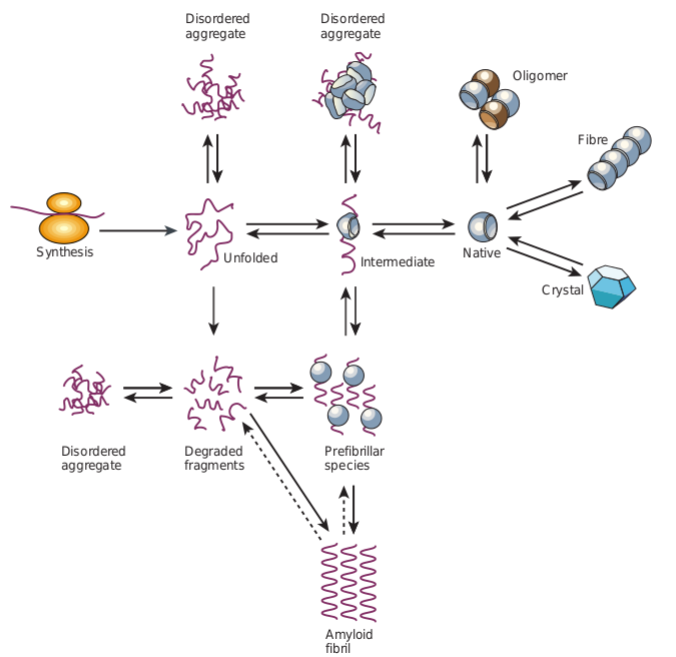
\includegraphics[width=\textwidth]{img/aggregationDiagram.png} 
\caption{Equilibrio de los estados de agregación} \label{aggregationDiagram}
\end{figure}



De la figura puede verse también, que pueden ocurrir distintos procesos de agregación, que resultan en disintas estructuras agregadas, a partir de distintas estructuras adoptadas por las proteinas.



% FIBRAS AMILOIDES: CARACTERISTICAS ESTRUCTURALES Y PROPIEDADES BASICAS
All amyloid fibrils share the same cross-beta archi-
tecture and several functional proteins found in bacte-
ria, fungi, insects and humans have also been found to
adopt the same architecture under physiological condi-
tions, as part of their functional role despite the diversity of origin of their
constituent proteins.













The critical step in the aggregation process is the unfolding of the native structure. 
En la mayoria de las proteinas, excepto las mas pequeñas, el 'unfolding' que ocurre en condiciones fisiologicas no lleva a una estructura totalmente desplegada sino que la proteina adquiere una estructura semi-estable parcialmente collapsada,
donde las interacciones no son las mismas que en el estado nativo estructurado, estas son caracteristicas propias de los intermediarios del plegamiento.

The energy landscape model suggests that some folding intermediates might have structural elements not present in the final folded state.
The appearance of such misfolded intermediates might initiate protein oligomerization or aggregation

La formacion de estos intermediarios es importante porque generalmente son mucho mas solubles que si se formaran conformaciones altamente desplegadas. 
Esta solubilidad permite alcanzar las concentraciones requeridas para la nucleacion propia de la formacion de amyloids(y de agregados en general????)













% ***********************************************************
% ******* PROPIEDADES DE FORMACION DE AMYLOIDS
% ***********************************************************


Since all fibrils independent of the original structure of the given amyloidogenic protein have a common cross-b structure, considerable conformational rearrangements have to occur prior to fibrillation. 
Such changes cannot happen in a native protein, due to its stable and rigid tertiary structure. Thus, protein destabilization favoring partial unfolding and culminating in the formation of a partially unfolded conformation is required. 
Presumably, such a partially unfolded conformation favors reciprocal and specific intermolecular interactions, including electrostatic attraction, hydrogen bonding and hydrophobic contacts, which are necessary for oligomerization and fibrillation
Obviously, this model does take into account a class of natively unfolded proteins, as they are devoid of rigid tertiary structure in their native state.

Data have been reported indicating that the first critical step in protein fibrillogenesis is the partial unfolding of the protein. 
Due to structural fluctuations (conformational breathing) the structure of a globular protein under physiological conditions represents a mixture of tightly folded and multiple partially unfolded conformations, 
with great prevalence of the former. 
Most mutations associated with accelerated fibrillation and protein deposition diseases have been shown to destabilize the native structure, increasing the steady-state concentration of partially folded conformers

Detailed structural analysis of early fibrillation events in several proteins has demonstrated that the amyloidogenic conformation is only slightly folded and shares many structural properties with the premolten globule state.

This picture enables us to speculate on the origins of the amyloid diseases from the point of view of the physico-chemical properties of the protein molecules. If
the stability or cooperativity of the native state of a protein is reduced, for example by a mutation, the population of non-native states will increase.
This rise will increase the probability of aggregation, as the concentration of polypeptide chains with at least partial exposure to the external environment will be greater. Whether or not aggregation does occur will depend on
the concentration of protein molecules, the intrinsic propensity for a given sequence to aggregate when unfolded, and on the rate of the aggregation process. The
fact that formation of ordered amyloid fibrils can be seeded, like the well-studied processes of crystallization
and gelation, means that once the aggregation process is initiated it often proceeds very much more rapidly.
In the absence of seeding there can be long 'lag' phases before aggregation occurs . This lag can be thought of as arising because the growth of a fibril cannot occur until a 'nucleus' of a small number
of aggregated molecules is formed. Such a nucleus can be formed by the local £uctuations in concentration that occur in solution as a result of random molecular motion. When such fluctuations result in a local concentration of
molecules above a critical value, the molecules associate with one other to form a species that is suficiently large to have intrinsic stability, and hence to grow in size by interacting with other molecules in the solution. The act
of seeding provides such nuclei to the solution and hence reduces or abolishes the lag phase

The proposal that amyloid fibrils are a generic structure of polypeptide chains (se desarrolla mas adelante en la parte de amyloids) coincide con esta forma de ver.

% The amyloid conformation reflects an intrinsic conformational propensity of polypeptides as many proteins can be forced into amyloid fibrils by manipulating external conditions. 
Several observations (por ejemplo que ordinary peptides and proteins can convert under appropriate laboratory conditions into aggregates with all the characteristics of the amyloid fibrils),
together with a wide variety of biophysical and computational studies, led to the suggestion that the amyloid structure can in principle be adopted by any polypeptide chain.
The amyloid state of a protein is therefore generic, as it is accessible to many different polypeptide chains, and, unlike the native state, its essential architecture is not encoded by the amino acid sequence,
although the details of its structure and stability can be markedly sequence-dependent, as we discuss below. 
% Despite active research, a detailed understanding of the molecular principles underlying the transformation of soluble proteins into amyloid aggregates is still lacking

% However, amyloid formation is also a sequence-specific process 14,15 .
Even though the ability to form amyloid fibrils seems to be generic, the propensity to do so under given circumstances can vary markedly between different sequences.
Under physiological conditions, most peptide sequences derived from proteins will remain soluble even at high concentrations, whereas most hydrophobic sequences will invariably aggregate as amorphous aggregates.

Similar to globular native states, amyloid structures are closely packed and highly ordered



Amyloidogenic proteins are quite diverse, with little similarity in sequence and native three-dimensional structure.
Additionally, several proteins and peptides not related to amyloidoses have the potential to form amyloid fibrils in vitro, suggesting that this ability for structural rearrangement and aggregation may be inherent to proteins.
Even though the ability to form amyloid fibrils seems to be generic(is a general property of the polypeptide backbone), the propensity to do so under given circumstances can vary markedly between different sequences(depends enormously on amino acid composition.).

This picture enables us to speculate on the origins of
the amyloid diseases from the point of view of the
physico-chemical properties of the protein molecules. If
the stability or cooperativity of the native state of a
protein is reduced, for example by a mutation, the popu-
lation of non-native states will increase.
This rise will increase the probability of aggregation, as the
concentration of polypeptide chains with at least partial
exposure to the external environment will be greater.
Whether or not aggregation does occur will depend on
the concentration of protein molecules, the intrinsic
propensity for a given sequence to aggregate when
unfolded, and on the rate of the aggregation process. The
fact that formation of ordered amyloid fibrils can be
seeded, like the well-studied processes of crystallization
and gelation, means that once the aggregation process is
initiated it often proceeds very much more rapidly.
In the absence of seeding there can be
long 'lag' phases before aggregation occurs .
This lag can be thought of as arising because the growth
of a fibril cannot occur until a 'nucleus' of a small number
of aggregated molecules is formed. Such a nucleus can be
formed by the local fluctuations in concentration that
occur in solution as a result of random molecular motion.
When such fluctuations result in a local concentration of
molecules above a critical value, the molecules associate
with one other to form a species that is suficiently large
to have intrinsic stability, and hence to grow in size by
interacting with other molecules in the solution. The act
of seeding provides such nuclei to the solution and hence
reduces or abolishes the lag phase







% **********************
% AGREGADOS AMORFOS
% **************************

Amorphous beta-sheet aggregation, is less position-dependent(than amyloid aggregation) and can, in principle, be achieved by any sequence that can adopt an extended conformation, is sufficiently hydrophobic and has no unsatisfied hydrogens or electostatic groups. 
Thus beta-sheet aggregation can be relatively easily predicted by methods that evaluate aggregation by evaluating biophysical parameters over a sequence segment, without the need for considering position-dependent values of these parameters.





% AGREGACION DE PROTEINAS IDPs

%Many proteins adopt various other biologically relevant conformational states in addition to their native structure. 
%These partially folded protein species are particularly vulnerable to misfolding and aggregation from which they must be protected in living systems

Intrinsically disordered proteins are not necessarily prone to aggregation, as their sequences have usually evolved to maintain the level
of solubility that is required for their optimal function; for example, through the existence of extensive regions that are highly abundant in charged and polar groups
that disfavour intermolecular association from a thermodynamic point of view. 
Moreover, as is discussed below, kinetic barriers to aggregation are crucial in enabling both globular and disordered proteins to maintain their soluble and functional states





% FUNCTIONAL AMYLOIDS
Amyloids are not only associated with disease-related proteins.
Nature also exploits the structural and mechanical properties
of amyloids to regulate biological functions 13 . For example, in
bacteria amyloids such as curli promote biofilm formation and
host invasion, and chaplins in bacteria and hydrophobins in yeast
act as regulators of surface tension of water. Insects and fish
use chorion amyloid as a component of eggshell, and spiders
use spidroins in spider silk. Humans possess at least one func-
tional amyloid protein: Pmel17 is used as a structural scaffold
in melanin synthesis. The strength and flexibility of amyloids
have attracted attention for their use as biomaterials. However,
it remains to be understood how functional amyloids avoid the
cytotoxic effects observed in disease amyloids. In part, functional
amyloids are regulated by chaperones and proteases. But it is
also becoming evident that sequence composition modulates
critical biophysical parameters determining kinetics of assembly
or mechanical strength.




\subsubsection{Mecanismos naturales de proteostasis}
En secciones previas(en la introduccion) se dijo que el espacio de conformaciones accesibles por las proteinas dependia de las estabilidades termodinamicas de los estados y la cinetica de interconversión entre estos. 
Estas propiedades, a su vez, dependen del contexto celular en el que se encuentran(ademas de la secuencia de la proteina en si misma), concentraciones de proteinas, localizacion, interacciones, etc.
El balance correcto entre todas estas condiciones está regulado a traves del proceso de proteostasis.
Proteostasis refers to controlling the concentration, conformation, binding interactions (quaternary structure), and location of individual proteins making up the proteome by readapting the innate biology of the cell, 
often through transcriptional and translational changes.
The protein components of eukaryotic cells face acute and chronic challenges to their integrity. Eukaryotic protein homeostasis, or proteostasis, enables healthy cell and organismal development and aging and protects against disease
Los mecanismos dentro del proceso de proteostasis permiten successful organismal development and aging in the face of constant intrinsic and environmental challenges %previniendo el desarrollo de enfernedades.

The healthy state of a cell is characterized by a detailed balance between the different states that proteins can populate. 
Perturbations to such balance, unless they are kept under strict control, can lead to deleterious events and disease.


La proteostasis es influenciada por todos los mecanismos que controlan los aspectis vistos en las secciones previas..... by the chemistry of protein folding/misfolding and by numerous regulated networks of interacting and competing biological pathways 
that influence protein synthesis, folding, trafficking, disaggregation, and degradation.

La celula posee distintos mecanismos para regular estos procesos .....chaperonas para regular el proceso de folding/misfonding (y tambien de aggregation), 
Nature developed very sophisticated protection mechanisms (chaperones, proteasome, etc.) for the effective regulation of the folding process, y por lo tanto prevenir las peligrosas consecuencias de misfolding. 
In other words, in the cell, any given protein is not acting in the isolation, is never alone and is
constantly "watched" by the protective machinery. This machinery is rather robust and can
tolerate significant loads. Obviously, factors that affect these protective mechanisms will
contribute to the probability of disease development


-Cells possess a complex proteostasis network (PN) to ensure protein homeostasis.
-Aggregates permanently engage molecular chaperones and other PN components.
-The PN is challenged by chronic stress in protein-aggregation diseases and aging.
-Overtaxing the PN drives a vicious cycle of disease progression with eventual proteostasis collapse.



Las diferencias estructurales vistas entre los distintos estados de agregación tambien se ven reflejada en diferencias biológicas 
Whereas misfolded and aggregated proteins are found in perinuclear locations and are generally degraded by the 
proteasomal system, amyloids preferentially accumulate in perivacuolar inclusions, where they are degraded by the autophagosome.
% This segregation directly results from a differential recognition by the protein quality control system. 
Esta segregación resulta en un tratamiento distinto por parte de los mecanismos encargados de la proteostasis.
A reduced affinity of amyloids for the protein quality control system is probably also at the root of their higher toxicity 11 as artificial overexpression of chaperones
usually leads to decreased toxicity and removal of amyloids from he cell.
Contrary to amorphous aggregates, amyloid structures can fulfill biological functions, and functional amyloids are found in organisms from prokaryotes to humans \cite{fowler2007functional}.





% PREVENCION DE AGREGACION EN FOLDED PROTEINS
the normal folding process may pass through
partially folded states on the route to the fully native state,
but the aggregation of these species will be minimized by
the presence of molecular chaperones. In addition, if the
protein is able to fold rapidly, any partially folded species
will have a short lifetime, reducing the probability of inter-
molecular interactions occurring. Moreover, once folded,
the native state is generally a highly compact structure
that conceals the polypeptide main chain within its
interior. Such a state is protected from aggregation except
through the interactions of surface side chains (as is the
case, for example, in protein crystals) and is unable to
form the strong intermolecular hydrogen bonds associated
with the polypeptide backbone. Provided that the native
state is maintained under conditions where it remains
folded, aggregation to amyloid fibrils will be resisted by
the kinetic barrier associated with unfolding, even if the
aggregated state is thermodynamically more stable.
Importantly, the cooperative nature of protein structures
means that virtually none of the polypeptide chain in indi-
vidual molecules is locally unfolded, and that virtually no
molecules in an ensemble are globally unfolded, even
though native proteins are only marginally stable relative
to denatured ones under normal physiological conditions


% ACA EXPLICO POR QUE LAS IDPs NO TIENEN TANTA TENDENCIA A FORMAR AGREGADOS
In contrast to the globular proteins, which have to unfold prior to aggregation (Jahn and Radford, 2005), IDPs are always ready for intermolecular interactions. 
An unbound fragment of an IDP possesses a strong ability to interact, and therefore can bind either to natural partners forming native complexes or to similar molecules forming various aggregates. 
This raises the question of why IDPs do not always form aggregates in the norm. One of the potential answers is the fact that inside the cell, the IDPs typically form complexes with natural partners.
Los mecanismos de proteccion (chaperonas, proteasoma, etc) tienen una gran capacidad para mantener la solubilidad de proteinas.
Además, based on the analysis of the IDP amino acid composition, it would be clearly a mistake to assume that an averaged IDP possesses higher propensity towards aggregation than an averaged ordered
protein. In fact, many IDPs contain large number of charged and polar residues. In addition to the hydrophobic interactions, the net charge is one of the major factors determining aggregation behavior of a protein.













\subsection{Características funcionales}
\label{functionalLandscape}
\begin{itemize}
 \item Breve historia estructura-función
 \item motivos secuenciales
 \item funcionalidad en proteinas IDPs
\end{itemize}

% PRIMERO HABLAR DE DOMINIOS GLOBULARES.....
Dado que en dominios globulares la estructura esta definida y esta asociada a la funcion que desarrolla la proteina, este estructura puede ser usada para clasificacion y para inferir la funcionalidad en nuevas proteinas.
% PFAM, SCOP


One of the best-
understood functions of proteins is catalysis (i.e., enzymatic
activity), which attracted much attention in the early days of
protein science and led to the elaboration of the “lock and key”
model by Fisher. Central to this model is the notion that the
correct shape of the substrate can fit into the active site of the
enzyme for enabling an efficient and specific catalysis,






% HASTA ACA DEBERIA HABER DEFINIDO TODOS LO QUE RESPECTA A ESTRUCTURA-FUNCION EN DOMINIOS GLOBULARES

Estos dominios globulares pueden ser identificados y asociados a una funcion individual o a una funcion dentro de la funcion global de la proteina.
Domains are now readily detectable with sequence
searching programs (e.g., Blast [9] or HMMer [10]) and readily
alignable by standard methods (e.g., ClustalW [11] or MUS-
CLE [12]). Known domains are now stored in a number of dat-
abases including Pfam [1], SMART [13], CDD [14] and
InterPro [15] and remain a critical component of genome
annotation procedures. Particular domains and domain archi-
tectures are well conserved over the course of evolution (e.g.,
Fig. 1). The sequences diverge, but the overall domain archi-
tecture remains the same.




% FUNCIONALIDAD EN IDPs

% DEBERIA PRIMERO INTRODUCIR EL CONCEPTO DE QUE LAS IDPs TAMBIEN PUEDEN CUMPLIR FUNCIONES
% DESARROLAR HASTA LLEGAR A LA PREGUNTA CLAVE DE  COMO ES EL MECANISMO Y CUALES SON LAS FUNCIONES QUE CUMPLEN
% DESPUES PONGO EL CUADRO QUE DESCRIBE LOS MECANISMOS, TANTO DE IDPs COMO DE PROTEINAS FOLDED  
% \begin{figure}[h!,centered]
% \centering
% 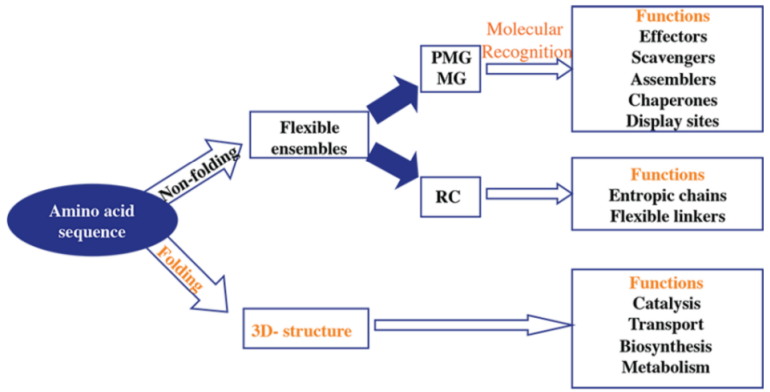
\includegraphics[width=0.7\textwidth]{img/proteinFunctionMechanisms.png} 
% \caption{Distinctive properties of proteins: diversity and functional role }
% } \label{proteinMechanisms}
% \end{figure}

% DESCRIBO BREVEMENTE ESOS MECANISMOS 
% HABIANDO DESCRITO LOS MECANISMOS SE DEDUCE QUE GRAN CANTIDAD DE ESTOS ESTAN RELACIONADOS CON MOLECULAR RECOGNITION
% PUEDO PONER ESTE TEXTO: 
% As also apparent from the foregoing classification, IDPs often
% function via molecular recognition, when they bind partner
% molecules in, and induced folding process. Their mode of
% binding is thought to confer many advantages, and is often
% mediated by short recognition elements (motifs)

% UNA VEZ DESCRITO ESTO PUEDO DESARROLLAR EL TEMA DE SLM, Y FINALMENTE LO ASOCIO CON EL TEMA DE MoREs , AHI CITO AL TRABAJO DE \cite{fuxreiter2007local}





However, domains are only part of the picture. Many studies
have shown that they cover only a fraction of the protein se-
quence contained in an organism. The remaining parts of the
sequence only rarely contain undiscovered domains, and in-
deed have been shown to be low-complexity (i.e., dominated
by a few amino acids) or intrinsically disordered (see [3] for re-
view).A fraction of these regions are likely linkers that permit
the correct spacing of domains in a functional protein, though
many others are known to play pivotal functional roles. 
Critical sites for phosphorylation,
or other modifications often
lie within them, as do regions important for interactions with
other proteins. These very short, functional regions, though
not globular domains, often conform to particular sequence
patterns or linear motifs indicative of a particular function

In the sense that they are modular, or repeated in many dif-
ferent contexts, linear motifs are similar to domains. However,
they differ in one critical aspect: whereas domains are now ac-
cepted only to arise by gene duplication, linear motifs, because
of their short length, can easily arise convergently.


The rationale of the connection between LMs(linear motifs) and intrinsically unstructured/disordered proteins(IUPs/IDPs), is that the latters are frequently associated with
regulatory functions in signal transduction or transcription in eukaryotic proteomes. These functions are carried out by molecular recognition that is linked to a binding-coupled
folding process
% ESTA ES LA BASE DE LA RELACION, Y DESPUES SE COMPROBO QUE EFECTIVAMENTE LA MAYORIA DE LOS LMs CAEN EN REGIONES IDPs/IDRs



% ESTO ES MASOMENOS LO MISMO QUE LOS ULTIMOS 4 PARRAFOS, MERGEAR TODO............

However, there remain protein sequence segments that are difficult to analyse productively. 
For example, there are often large segments of multidomain proteins that are non-globular, intrinsically lacking the capability to fold into a defined tertiary
structure (9–11). Sometimes the function of such regions may be as simple as linkers connecting globular domains and the sequence of amino acids is not important.

Very often, however, these unstructured regions may contain functional
sites such as protein interaction sites, cell compartment target-
ing signals, post-translational modification sites or cleavage
sites. These sites are usually short and often reveal themselves
in multiple sequence alignments as short patches of conserva-
tion, leading to their definition as short sequence motifs. In
addition to occurring outside globular domains, some sites, for
example, phosphorylation sites, are often found in exposed,
flexible loops protruding from within globular domains

The PROSITE database has collected a number of linear
protein motifs, representing them as regular expression
patterns (5).


% Este concepto de regiones desordenadas que cumplen funciones especificas se puede extender a proteinas enteras.
% “intrinsically disordered” proteins
% (IDPs) or regions (IDRs),
% possess no well-defined 3-D structure but rather adopt an
% ensemble of conformations in solution, yet they are functional.

% En las secciones anteriores se mostro como es la realidad en cuanto a la conformacion de proteinas en su estado nativo, 
% entre las cuales podemos encontar gran variedad de proteinas funcionales que no adoptan una estructura tridimensional definida
% y por lo tanto no se ajustan a este paradigma de estructura funcion, aunque si se sabe que cumplen funciones celulares relevantes.



% ACA YA SE SOBREENTIENDE QUE LAS IDPs/IDRs PUEDEN TENER FUNCIONALIDADES

El proteoma funcional es el resultado, entonces, tanto de dominios con estructura definida como de proteinas IDPs \ref{stuctured-idp-functions}

Protein sequences in a genome can be viewed as modular because they are made up of combinations of structured and disordered regions.
Proteins without IDRs are called structured proteins, and proteins with entirely disordered sequences that do not adopt any tertiary
structure are referred to as intrinsically disordered proteins (IDPs). 
The majority of eukaryotic proteins are made up of both structured and disordered regions, and both are important for the
repertoire of functions that a protein can have in a variety of cellular contexts.

Thus, functional regions in proteins can
either be structured or disordered, and these need to be
considered as two fundamental classes of functional building
blocks of proteins


\begin{figure}[h!,centered]
\centering
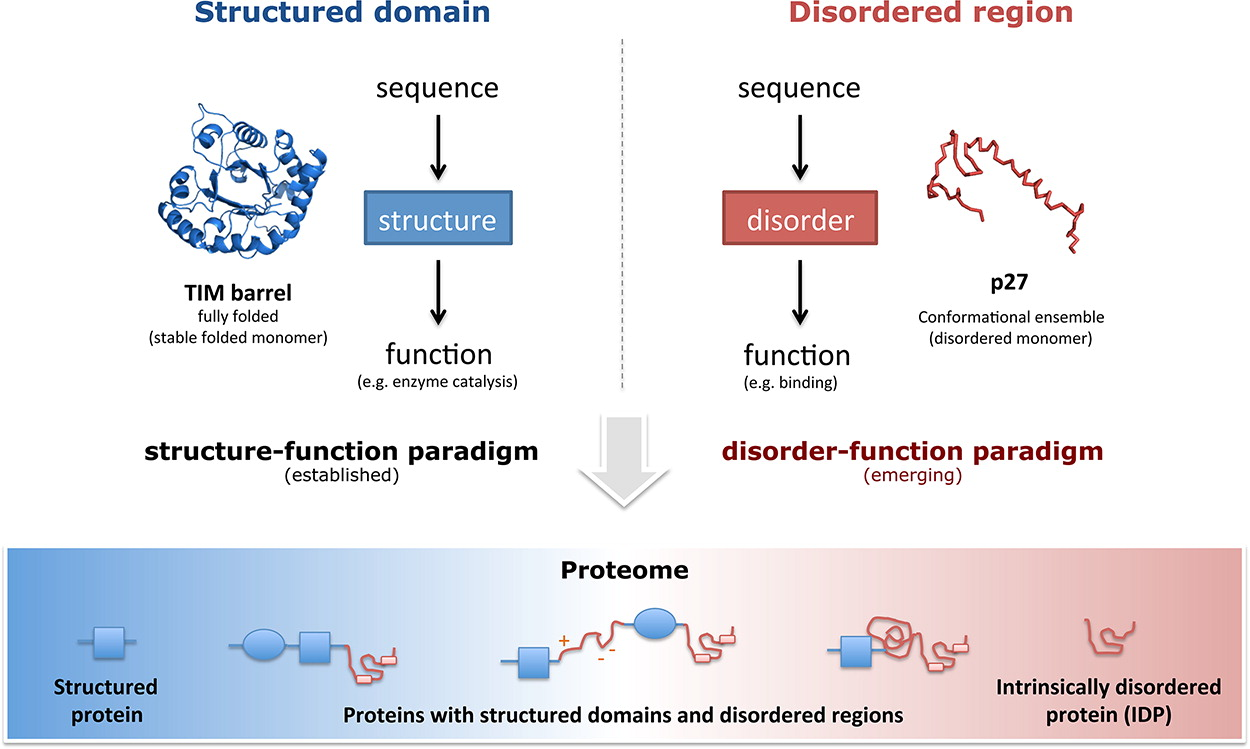
\includegraphics[width=0.9\textwidth]{img/structure-idp-function.jpeg} 
\caption{Paralelismo entre funcionalidad emergente de dominios plegados y de proteinas IDPs. Figura extraida de \cite{van2014classification}}
\label{stuctured-idp-functions}
\end{figure}


This means that the structure-function paradigm, which emphasizes that ordered 3D structures represent an indispensable prerequisite to effective protein functioning, should be redefined to include intrinsically unstructured proteins [159]. 
According to this redefined paradigm, native proteins (or their functional regions) can exist in any of the known conformational states, ordered, molten globule, premolten globule and coil. 

To accommodate all these states in a functional framework, Keith Dunker elaborated the protein trinity hypothesis, 82 which posits that a native protein can be in one of three states -the ordered state, the collapsed-disordered
(molten globule, MG) state, and the extended-disordered state (random coil, RC)- and that function can arise from any of the
three states or from transitions between them. 82 This model was subsequently expanded to include the premolten globule (PMG)
state, which corresponds to an intermediate state between the RC and the MG (Figure 9) 13

Function can arise from any of these(cuatro) conformations and transitions between them \ref{proteinQuartet}. Thus, not just the ordered state but any of the known polypeptide conformations can be the native state of a protein.

The ultimate goal of the structural description of IDPs is to elucidate and rationalize the types and modes of functions they play.
The most important question of the field, therefore, is the physiological function and functional mode of IDPs/IDRs.


% TODO ESTO QUE ESTA COMENTADO HABLA DE CUALES SON LAS VENTAJAS QUE TIENEN LAS IDPs PARA REALIZAR CIERTAS FUNCIONES
%  Y LAS FUNCIONES QUE TIENEN MAS VENTAJAS DE SER IMPLEMENTADAS POR IDPs

% The functional role of structural disorder from a biological process view addresses what type of cellular functions benefit most from the lack of a stable structure. This question was addressed in several large bioinformatics studies. 
% As a result, IDPs are generally thought to be involved in processes of signaling and regulation, and in depth correlation analysis [52] of 710 Swiss-Prot functional keywords suggested significant positive correlation with 238 functions and negative correlation with 302 functions (Table 2). 
% Most of the functions that correlate with the presence of long disordered regions are related to regulation via transcription and translation, whereas functions that correlate with the lack of disorder are dominated by enzymatic catalysis.
% 
% Algunas propiedades interesantes de las proteinas IDPs se revelan a partir de estudios a nivel de proteoma y sistema.
% As a result of breathtaking advances in comparative evolutionary and experimental structure–function studies, it is now clear that the intrinsic lack of structure and function-related disorder-to-order transitions provide
% IDPs with various functional advantages\cite{gunasekaran2003extended,dyson2005intrinsically}, such as: (i) Decoupled specificity and strength of
% binding provides for high-specificity-low-affinity interactions; 
% (ii) Increased speed of
% interaction due to greater capture radius(and it can bind at a relatively larger distance
% followed by reeling on to the partner, potentially enhancing
% the rate of binding by a ‘fly-casting’ mechanism, according to which the unfolded polypeptide first binds weakly at a relatively large
% distance from the actual binding site and then folds as the protein approaches the binding
% site)
% and the ability to spatially search through
% interaction space (ie. in the spatial search by transcription factors
% in sequence-specific DNA recognition, termed the ‘monkey-
% bar’ binding mechanism);
% (iii) Increased interaction (surface) area per residue; (iv) The ability for
% one-to-many and many-to-one interactions; (v) Increased capture radius for a specific
% binding site in comparison with that of ordered protein with its restricted conformational
% freedom, (vi) Fast binding kinetics, etc

% Intrinsic plasticity has been proposed to be advantageous because it could enable a single protein to recognize many biological targets while still being specific
% Moreover, it has been pointed out that the susceptibility to proteases and, hence,
% shortened lifespan of disordered proteins is an added advantage because these proteins play roles in cell-cycle
% regulation
% 
% 
% Ademas, Disordered proteins often have large intermolecular interfaces, the size of which is dictated by protein function. For proteins to be stable as
% monomers with extensive interfaces, protein size would need to be 2–3 times larger. This would either
% increase cellular crowding or enlarge the size of the cell by 15 –30\%, owing to the increase in the sequence
% length. Smaller sizes of cells, proteins, DNA and RNA conserve energy. Thus, disordered proteins provide a
% simple yet elegant solution to having large intermolecular interfaces, but with smaller protein, genome and
% cell sizes. The natively disordered state is a simple and elegant solution adopted by evolution to avoid large protein, genome and cell sizes.

% For many examples, the given disordered regions are not known to bind to any partner, but they still carry out
% important functions such as providing flexible linkers be-
% tween structured domains or providing flexible tails that
% regulate the structured domains

% Several of their specific functional modalities, such as adaptability in binding, high functional density, weak but specific binding, and frequent regulation by post-translational modification, have been formally demonstrated. 
% 
% 
% Even if the lifetime of the preferred native
% conformation is short(como es el caso de las disordered conformations), this conformation still exists. The
% binding and shift in the equilibrium takes care of
% the function.




% PROPIEDADES Y MECANISMOS FUNCIONALES

El estudio de las funcionalidades provistas por IDRs y IDPs se ve dificultada por las propiedades intrínsecas de estas proteinas:
Given the absence of structural constraints, IDRs tend to evolve more rapidly than protein domains that adopt defined structures. As a result,
identifying homologous regions is harder for IDRs and IDPs than it is for structured domains.
This complicates the transfer of
information about function between homologues and thus the
prediction of function of IDRs and IDPs.

these
considerations raise the need to devise a classification scheme
specifically for disordered regions in proteins that may enhance
the function prediction and annotation for this important class of
protein segments.

Aun cuando las propiedades a clasificar no sean discretas sino que formen un continuo de opciones, es util para explicar y entender mejor los conceptos.
En secciones anteriores(mas precisamente en la seccion sobre propiedades conformacionales) se hicieron clasificaciones sobre la estructura global de la proteinas/regiones desordenadas, 
ademas se clasificaron los mecanismos de binding en este tipo de proteinas como conformational selection and induced folding
Especificamente se hablara aqui de clasificaciones sobre las funcionalidades y mecanismos funcionales provistos por estas proteinas.

En la figura \ref{proteinMechanisms} se ve una clasificación general bastante simplificada de los roles y mecanismos funcionales generalmente provistos por los distintos tipos de proteinas. 
En esta clasificacion de proteinas segun su rol general, se incluyen también los dominios/proteinas plegadas que mencionamos previamente.

\begin{figure}[h!,centered]
\centering
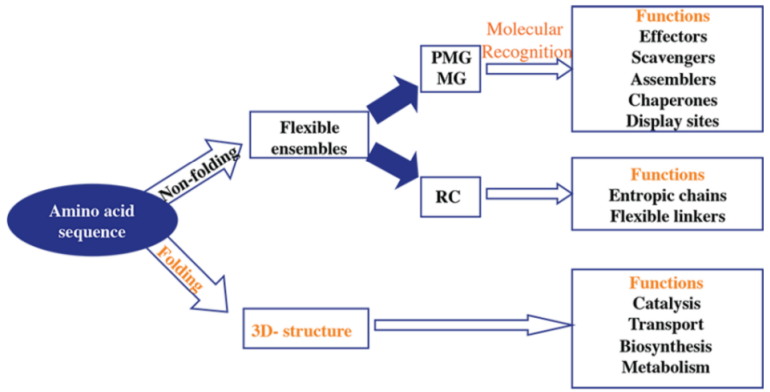
\includegraphics[width=0.9\textwidth]{img/proteinFunctionMechanisms.png} 
\caption{Distinctive properties of proteins: diversity and functional role. Figura extraida de \cite{habchi2014introducing} }
\label{proteinMechanisms}
\end{figure}


En la figura \ref{idpFunctions} se detalla la clasificacion de funcionalidades y mecanismos funcionales para IDPs/IDRs.


Como parte de estos avances para intentar dilucidar las funcionalidades de las IDPs y sus mecanismos asociados, se han intentado organizar y clasificar las funcionalidades provistas por estas \cite{van2014classification}.


\begin{figure}[h!,centered]
\centering
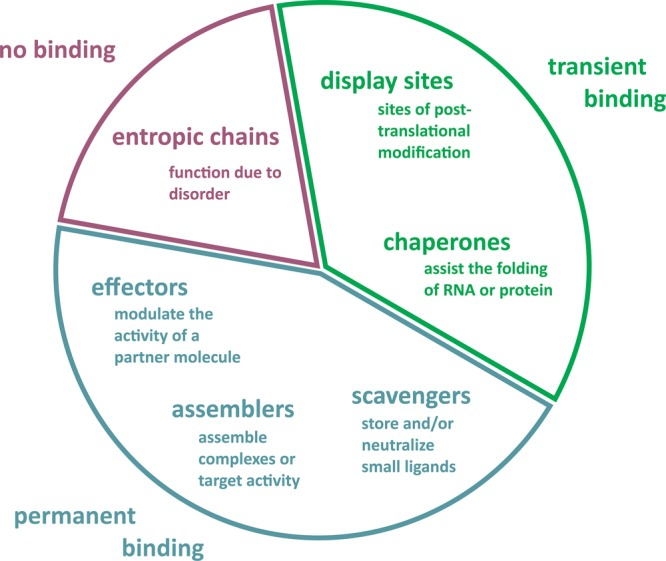
\includegraphics[width=0.9\textwidth]{img/idpFunctionMechanisms.jpg} 
\caption{Clasificación roles y mecanismos funcionales de IDPs/IDRs. Figura extraida de \cite{van2014classification}}
\label{idpFunctions}
\end{figure}


Como se puede ver en la figura \ref{proteinMechanisms}, IDP functions either directly stem from their disorder (entropic chains where function
involves no coupled binding and folding; rather it directly depends on the flexibility and the plasticity of the backbone, 
or from molecular recognition mechanisms , when they undergo induced folding (disorder-to-order transition) upon binding to a partner molecule.


Para entender mejor las funcionalidades, intentaremos ahora hacer una clasificacion de las functional features(modulos funcionales) que pueden encontrarse dentro de IDRs/IDP:

% As also 
apparent from the foregoing classification, IDPs often
function via molecular recognition, when they bind partner
molecules in, and induced folding process. Their mode of
binding is thought to confer many advantages %REFERENCIA AL PAPER DE MECANISMOS FUNCIOMNALES DE IDPs
, and is often
mediated by short recognition elements (motifs)\cite{neduva2005systematic,fuxreiter2007local,davey2012attributes}.


En las secciones previas se desarrollaron los conceptos de MoREs y PSE como elementos que se han descubierto desde el punto de vista estructural, podían conferir ....

% ACA CONECTO CON SLM
Sin embargo, molecular recognition by short recognition elements (motifs)
can be -and has been historically- approached from the
completely different direction of short sequence patterns
determining functional interactions and enzymatic modification,
i.e., LMs, ELMs, and SLiMs


% PUEDO DESARROLLAR LOS CONCEPTOS SOBRE SLMs ACA O PONER PRIMERO ESTOS PARRAFOS 


 
% ACA DIGO QUE, A PESAR DE TENER DIFERENCIAS, LOS SLMs Y LOS MoREs SON LO MISMO BASICAMENTE
% 

A measure that is often used to distinguish the different types of
disordered binding modules is length.

Ademas..MoRFs differ from ELMs and SLiMs in not depending on a specific sequence motif, but rather upon a pattern in a disorder prediction output. 

Although there are differences in the definitions of linear
motifs and MoRFs, they share many common features 72,163
including a tendency to undergo disorder-to-order transition (all
MoRFs by definition and aprox. 60\% of LMs 48 ), an enrichment in
IDRs (MoRFs by definition and aprox. 80\% of LMs are in IDRs 48,72 ),
and a tendency to promote complex formation.



Yet, interestingly, recent analysis suggests that linear motifs (LMs) (thus not differentiating between ELMs and SLiMs) show high overlap with MoRFs \cite{fuxreiter2007local}
A pesar de las diferencias que podremos encontrar entre los . Los últimos trabajos que se han hecho sobre el tema \cite{meszaros2012disordered, fuxreiter2007local} 
parecen indicar que .....
The overlap between linear motifs and MoRFs
especially, but also IDDs, suggests that these functional features
are different states in the same continuum of binding
mechanisms involving disordered regions.
% Different concepts regarding short recognition elements have
% been extensively discussed in the literature. Indeed,
depending
on whether the idea is approached from a structural point of view
or defined at the sequence level, a short motif could be denoted
as a “molecular recognition element” (MoRE)/“molecular
recognition feature” (MoRF) , a PSE, or “linear motif” (LM),
respectively (LM is also denoted as “eukaryotic linear motif”
(ELM) or “short linear motif” (SLiM)).


Whereas LMs have been identified as short sequence motifs critical in recognition functions, primary contact sites, preformed structural elements and molecular recognition elments/features have been approached from the direction of protein disorder, emphasizing recognition segments embedded in such regions. Unity of these concepts is underlined by the key role of a few specificity determinants in all these recognition elements, and also by their local preferences for undergoing disorder-to-order transition upon molecular recognition, which might already
be manifested prior to binding. 
Apart from a minority of the cases when LMs are constituted of segments of ordered domains, these different concepts of short recognition elements express the same underlying physical and
functional principles that provide a probably widespread solution to the dynamic control of protein-protein interaction networks.





% ACA AGREGO OTRO ELEMENTO, LOS DOMINIOS ID, QUE PUEDEN SER OTRA CLASIFICACION
Binding by motifs is usually weak, transient, and possibly of limited
specificity [39], which can be made stronger and/or more
specific by either cooperating with flanking regions, com-
bining several motifs, or utilizing longer disordered
domains

It is to be noted, however, that binding regions within IDPs
might correspond more to a domain than a motif, with their
lengths exceeding 20-30 residues \cite{tompa2009close,chen2006conservation,chen2006conservationB}  
Por lo tanto, estos pueden clasificarse como un elemento independiente que puede encontrarse dentro de IDPs (llamados intrinsically disordered domains (IDDs))
Indeed, these regions
possess typical characteristics of domains: (1) they are
structurally and functionally independent of the remainder of
the protein molecule, (2) they can be recognized by homology
due to evolutionary conservation of sequences, and (3)
they possess at least one specific function.

Potein domains with
conserved disordered regions have a variety of functions, but are
most commonly involved in DNA, RNA, and protein binding

A pesar de tener una longitud (al parecer) bastante mayor,
intrinsically disordered domains (IDDs) can also have significant
overlap with MoRFs and linear motifs







Though disordered interaction modules encompass a continuous range of binding interfaces, they can be approximately split into
three major classes of autonomous functional interfaces: 
- large serpentine disordered domains (e.g. CREB-binding protein (CBP) TAZ domain-binding modules in Hypoxia-inducible factor 1a 7 ), 
- multi-partite disordered interfaces (e.g. Inhibitor-2 binding to Protein phosphatase 1 8 ), and 
- compact mono-partite, short linear motifs (SLiMs) (e.g. the canonical SH3 domain-binding PxxP motif 9 ).





















% A PARTIR DE ACA ES TODO SOBRE SLMs, etc....

% PRIMERO DEBERIA DECIR UN POCO SOBRE SLMs DE FORMA INDEPENDIENTE A IDPs , DECIR QUE SON Y COMO SE EMPEZARON A ESTUDIAR, EN QUE MOMENTO SE CRUZAN CON IDPs Y COMO SE PODRIAN RELACIONAR CON MoREs, PSEs

Although the notion of linear motifs has been around since
the mid-1970s (see [16–18] for review), the first clear example
of a motif paired to its receptor molecule was not described un-
til 1990, when the targeting signal KDEL was paired to the
ERD2 receptor [19].
Moreover, despite the availability of
many thousands of sequences, the discovery of linear motifs,
in contrast to domains, has remained difficult. Their short
length makes them difficult to detect using sequence compari-
son procedures that aid domain discovery. They are typically
discovered by difficult and time-consuming experimental pro-
cedures. This usually involves first identifying a set of proteins
sharing a common function (e.g., a common interaction part-
ner or targeting within the cell), and then gradually delineating
a short, common segment associated with this function
through a variety of experimental techniques.

For instance,
the SH3 ligand was first identified as a recurring sequence fea-
ture in signaling proteins [20]. As interacting partners of SH3
containing proteins were gradually identified, the interacting
region was eventually reduced to a 9–10 residue, proline-rich
segment [21], which suggested a mode of action ultimately con-
firmed by 3D structures (e.g. [21,22]


En la actualidad hay un total de 2,475 instancias de peptide motifs en la base de datos ELM,



The number of instances of peptide motifs is suggested to be large \cite{tompa2014million}
but the difficulties in their discovery
mean that only about two hundred  %*********************************************************************REVISAR ESTE NUMERO !!
linear motifs are known
compared to thousands of domains that might bind them.


Several resources are devoted to the annotation and/or detection of SLiMs, helping with the difficult but rewarding task of motif discovery [elm.eu.org , Prosite (10), MiniMotifMiner (11) and Scansite (12)].
Known motifs are now being catalogued by several resources
(elm.eu.org [4]; scansite.mit.edu [27]).


Short linear peptide motifs are used
for cell compartment targeting, protein–protein inter-
action, regulation by phosphorylation, acetylation,
glycosylation and a host of other post-translational
modifications.








% PONER CONCEPTOS GENERALES DE SLMs
% 

El reconocimiento de la importancia y la gran cantidad de instancias que hay de este tipo de elementos en el proteoma eucariotico ha llevado a estudiar mas extensamente las propiedades de estos \cite{davey2012attributes}

These short interaction interfaces (which we herein refer to as ‘‘peptide motifs’’ to include both binding
motifs and posttranslational modification (PTM) sites 
next section) are typically less than ten residues in length and
enable both high functional diversity and functional density to
polypeptide segments containing them. On evolutionary time-
scales, they can evolve very rapidly by appearing de novo or
conversely disappearing with equal rapidity, conferring excep-
tional evolutionary plasticity on the interactome.

The known instances of peptide motifs have been shown to
mediate a wide range of important cellular tasks
They typically fall into two major classes: binding motifs, which mediate interactions with globular domains, and
posttranslational modification sites, which are recognized and altered by modifying enzymes.

These distinct terms denote functional sites
that often occur within disordered regions of proteins. 

These two features in isolation or in combination
permit the interaction and recruitment of diverse proteins in
space and time, thereby facilitating regulation of virtually all
cellular processes

For binding motifs, amino acid sequence specificity determi-
nants can be described. These determinants are often discov-
ered by identifying recurring patterns (or motifs) of residues
from functionally equivalent peptide sequences. Posttransla-
tional modification sites are less homogeneous, and many
appear to lack specificity determinants outside of the modified
residue

Linear motif-domain interactions are a subset of induced fit interactions, where the templated structure is induced in a short peptide of only a few residues.
As a consequence of the small number of residues involved, such interactions tend to be transient and have low binding affinities.
Therefore, they are well suited for mediating functions that require a fast response to changing stimuli. 
A classical example is the dynamic interaction between a kinase and its phosphorylation site: the kinase domain needs to bind to the peptide, attach the phosphate, and then dissociate again, potentially to then go on to interact in a similar way with other substrates.

Binding motifs are on average 6–7 amino acids in length, with
only 3–4 core positions conferring the majority of the interaction
specificity. The limited binding
surface area results in low-affinity, transient, and modulatable
interactions, usually in the low micromolar range. PTM sites in
general have weaker intrinsic specificity determinants


As a result of the involvement of a small number of residues
in peptide motifs, these functional modules exhibit high evolu-
tionary plasticity, and they can arise de novo and evolve conver-
gently by one or a few mutations within disordered regions

Due to relying on a very few confined residues and limited structural constraints, may frequently arise and disappear by point mutations, and confer extreme adaptability to the interactome.

Key advantages of LMs reside in that they facilitate the communication between proteins by having less stringent requirements for association. 
The resulting lowaffinity complexes are characterized by fast on and off binding rates that may serve regulatory purposes.


The amino acid composition of the polypeptide segment in
which peptide motifs are embedded shows strong resemblance
to that of IDRs \cite{fuxreiter2007local}


The majority of known
binding motifs and tens of thousands of PTM sites have been
discovered in predicted disordered regions.
This preference likely reflects (a)
the accessibility of such motifs within disordered regions, which
allows recognition by their binding partner, and (b) the flexibility
of such motifs, which enables them to adopt a specific conformation upon binding 




% EFECTOS A NIVEL RED SEÑALIZACION/SISTEMA
As suggested, IDPs/IDRs often function by binding accompanied by induced folding (molecular recognition) [6–8] mediated by SLiMs/ELMs, and in several recent
works it has been shown that the functional and evolutionary agility of IDPs can be ascribed to the inclusion or exclusion of such motifs in RNA maturation; that is, by alternative splicing, alternative promoter usage, and RNA
editing, the alternative isoforms thus generated promote the functional diversification of the proteome
This mechanism can result in a change in diverse functional attributes, such as subcellular localization, protein–protein interaction, phase transitions and even opposing (dominant negative) function, as also demonstrated by
studying tissue-specific forms of alternative splicing. These protein isoforms tend to occupy central positions in interaction networks and their pattern of interaction partners tend to significantly differ [63]; that is, structural disorder
and encoded motifs have a strong potential to define and redefine wiring of cellular signaling pathways.



% 
% 
% ACA TERMINAN LOS CONCEPTOS GENERALES DE SLMs











% ACA HAY UN ASPECTO IMPORTANTE DE POR QUE TENEMOS QUE SACARLOS.
% COMO ESTAN DEFINIDOS POR UN PAR DE AAs PUEDEN APARECER CONVERGENTEMENTE Y DE HECHO SE ENCUENTRAN EN UNA GRAN CANTIDAD DE PROTEINAS DONDE EN REALIDAD NO SON FUNCIONALES
% SEGUN ENTIENDO, EN ESTAS PROTEINAS ESTAN PERO NO EJERCEN INTERACCIONES PARA CUMPLIR LA FUNCION
% ES DECIR, DE ALGUNA FORMA U OTRA LA NATURALEZA SE OCUPA DE QUE, CUANDO APARECEN EN UNA PROTEINA DONDE NO TIENEN QUE ESTAR, NO INTERFIERAN. ES DECIR, NO OCURRA BINDING CON PATRONES CUANDO NO ESTAN PARA ESTA FUNCION
% UNA FORMA ES MEDIANTE COMPARTIMENTALIZACION CELULAR, OTRA ES MEDIANTE EXPRESION DIFERENCIADA EN EL TIEMPO
% EMN NUESTRO CASO NO PODEMOS ASEGURAR NINGUNO DE ESTOS MECANISMOS Y POR LO TANTOD DEBEMOS QUITARLOS
The fact
that they are defined by only a handful (usually 2–4) fixed ami-
no acids makes them very likely to arise or disappear by muta-
tions. And indeed they do often occur readily throughout a
typical proteome.
Binding non-functional patterns might also
be avoided by cellular compartmentalization and temporal dif-
ferences in gene expression, but it remains unclear as to whether
these are enough to maintain interaction specificit























\section{Ingeniería de proteínas}
\label{proteinEngineering}
% CONCEPTOS MUY GENERALES DE INGENIERIA


% TERMINO DICIENDO
En este trabajo nos centraremos en conceptos de diseño de proteinas quiméricas, formadas por dominios estructurales independientes unidos por secuencias linker.





\subsection{Proteínas modulares}
\begin{itemize}
 \item proteinas multidominio
 \item breve definicion dominios como unidades estructurales - evolutivas/funcionales
\end{itemize}


Because single domain globular proteins are often, though not always, easy to crystallise, for a long time they dominated perception of typical protein structure (although fibrous proteins like collagen were of course well known).
Gradually, as protein
sequences have accumulated, the monodomain view of protein
structure has been replaced by the realisation that most proteins
are multidomain, at least in higher eukaryotes.



% PARTE DE ESTO ESTA REPETIDO EN LA PARTE DE PROTEINAS MODULARES.....
Como se puede ver en el trabajo \cite{neduva2005linear}.....
Proteins are usually modular, containing discrete regions each of which performs a different sub-function. 
The most widely known modular element is the protein domain. These are typically more than 30 residues in length and fold into an independent compact structure. 
More than 7000 domains are known [1], performing an enormous diversity of functions from catalysis during metabolism to cell–cell recognition in the
immune system. Domain duplication is now an accepted mechanism of evolution, and differences in domain architecture are often responsible for critical differences between organisms.
Duplications are thought to be followed either by loss of one copy or the evolution of a new function by point mutations.













The first X-ray crystallographic structures provided a static picture of protein architecture, but multidomain structures in multiple conformations were soon discovered, where individual domains were connected by flexible linkers.

% Many cellular processes involve proteins with multiple domains.
Many eukaryotic proteins are modular — that is, they contain independently folded globular domainsthat are separated by flexible linker regions. 

In the absence of their targets, modular proteins
often behave as ‘beads on a flexible string’, where the
function of the linker is, primarily, to enable a relatively
unhindered spatial search by the attached domains


Dentro de esta gran cantidad de proteinas modulares:

-Many multidomain proteins are homomultimeric i.e. contain multiple copies of a single type of structural domain: Arisen through internal duplication of complete domains. Fate of domains determined by similar rules to paralogous genes

-Many multidomain proteins are heteromeric: Example is plasminogen activator where a trypsin-like serine protease is joined to kringle, finger and EGF domains
May occur by fusion of two or more genes (chimeric proteins). Also known as modular proteins, with domains known as modules. 

Certain modules occur in a wide variety of hetero- and homomultimeric proteins:
Suggests mechanisms to facilitate duplication and dispersal
“Building blocks” of different types of multidomain proteins are known as mobile protein modules
Frequency of transfer and incorporation into new protein reflects fixation probability


The modular nature of proteins has many advantages, providing increased stability and new cooperative functions.
Other advantages include the protection of intermediates within inter-domain clefts that may otherwise be unstable in aqueous environments and the fixed stoichiometric ratio of enzymatic activity necessary for a sequential set of reactions
In terms of evolution, modularity increases evolvability by reducing constraints on adaptation and by allowing preexisting parts to function in new contexts for novel uses.

There are various uses of the word domain with respect to proteins. 
We can define a protein domain as an independent, evolutionary unit that can form a single-domain protein or be part of one or more different multidomain proteins. The domain can either have an independent
function or contribute to the function of a multidomain protein in cooperation with other domains. 
The definition of a domain as an evolutionary unit is used in the Structural Classification of Proteins (SCOP) database \cite{murzin1995scop}

In contrast with this, in CATH \cite{orengo1997cath}, domains are domains are defined on a purely structural basis.
De esta forma .........protein domains can be defined as segmented portions of a polypeptide sequence that assume stable three-dimensional structure.

The original definition was largely structural: domains were thought
to be spatially distinct, probably independently folding enti-
ties. The advent of modern molecular biology gave rise to
many thousands of DNA and protein sequences. Sequence
alignments showed that many long proteins shared shorter re-
gions of homology with others, and this gave rise to a defini-
tion of domains based more on sequence recurrence, usually
also associated with some common function (e.g., catalysis
or binding). 

% There are
% now several globular protein domain databases accessible on
% the web, including Pfam (3), SMART (4), PROSITE (5),
% INTERPRO (6), PRODOM (7) and BLOCKS (8). 
Using these
tools, a user can often get a good overview of the domain
architecture of a polypeptide sequence and the functions these
domains are likely to perform.




Folded structures of proteins that are larger than 200-300 residues generally consist of multiple structural domains:
Domains are compact, stable units with a unique three-dimensional structure. 
Interactions within a domain are more significant than those between domains
Domains fold independently i.e. structural domains are also folding domains. If domain performs distinct function which remains intact in the isolated domain, then it is also a functional domain




Such recurring protein motifs are significant because it is increasingly recognized that there are only a limited number of domain families in nature.









These domains are duplicated and combined in different ways to form the set of proteins in genomes. 
The importance of domains is further exemplified by the fact that multidomain proteins play a major role in many cellular processes.

Although a consensus in detail is still lacking, various effective criteria have been proposed to detect and define protein domains.
These criteria rely mainly on the existence of local structural compactness arising from beta-sheets or hydrophobic cores. 
Based on such compactness, computational algorithms to detect structural domains have been proposed








\subsubsection{Secuencias linker naturales}
Estructura - Composición -  Estudios sobre linkers naturales


El 'descubrimiento' de las regiones/secuencias linkers esta ligado a las teorias de structura-funcion(desarrolladas en la parte de conformacion) que se dieron durante casi 100 años
En un principio se comenzo a pensar en una estructura rigida asociada a la proteina, luego se fueron revelendo propiedades dinamicas que le permitian cumplir la funcion. 
Todo esto esta muy asociado a las tecnicas experimentales que se fueron desarrollando.

Los primeros estudios de analisis (estructura y composicion) de secuencias linkers se comenzaron a hacer a partir del analisis estadistico de secuencias que podian ser clasificadas como linkers a partir de estructuras/secuencias almacenadas en bases de datos de proteinas.
Estos estudios estaban sesgados por todo el proceso historico de descubrimiento marcado por el modelo de estructura-funcion de las proteinas, y el concepto de hinge-bending.

The concept of hinge-bending, whereby the relative flexibility of short regions of the polypeptide chain allows significant movement of structural domains, gained widespread acceptance in
the 1980s and early 1990s, after evidence for conformational transitions in identical or homologous proteins became known.


En esos años, many studies of linker peptides in various protein families have come to the conclusion that linkers lack regular secondary structure, they display varying degrees of flexibility to match their particular biological purpose and are rich in Ala, Pro and charged residues

A lo largo de los años los conocimientos sobre la composición y propiedades de estas secuencias ha ido cambiando, 
a medida que mayor cantidad de estructuras se resolvian y mayor conocimiento se obtenia acerca de los dominios que componen las proteinas(ademas tambien influyeron otras cosas como tecnicas de biofisica para obtener informacion estructural en solucion, o algoritmos para automatizar la identificacion de la secuencia que actua como linker en una proteina)

Although the role of linker sequences is likely to be primarily topological, allowing distant parts of the polypeptide chain to interact with diverse partner sequences that might be far apart or close together, linkers and unstructured tail sequences play quite specific roles in a
number of systems

Hoy en dia, solo se puede decir que los linkers naturales son secuencias que actuan como espaciadores entre los dominios de una proteina, de manera que se prevengan interacciones unfavourable between folding domains. 
Esto solo se puede decir acerca de su definicion, ya que las propiedades dependen de la arquitectura de la proteina.

En \cite{george2002analysis} se hace un analisis sobre un dataset compuesto de toda una base de datos de proteinas, a partir de la cual se extraen los linkers.


En cada proteina, la secuencia linker puede tener una estructura y una funcion que haya sido seleccionada para el mecanismo/localizacion/funcion/etc de la proteina como un todo, y esta funcion del linker puede no ser solamente la union covalente de dos dominios para proveer increased stability and new cooperative functions.
Algunos linkers can play an essential role in maintaining cooperative inter-domain interactions
De esta forma, es dificil hacer un analisis y una clasificacion concreta de todos los linkers. Si se pueden agrupar algunos segun distintas caracteristicas funcionales, estructurales, etc.



Both flexible and relatively rigid peptide linkers are found in many multidomain proteins. 
Linkers are thought to control favorable and unfavorable interactions between adjacent domains by means of variable softness
furnished by their primary sequence. Large-scale structural heterogeneity of multidomain proteins
and their complexes, facilitated by soft peptide linkers, is now seen as the norm rather than the
exception. Biophysical discoveries as well as computational algorithms and databases have
reshaped our understanding of the often spectacular biomolecular dynamics enabled by soft linkers.
Absence of such motion, as in so-called molecular rulers, also has desirable functional effects in
protein architecture.

% *******************************************
% \subsubsection{Hinge-bending regions}
% ********************************************

It was discovered that hinge regions are
soft-linker regions of localized torsion angle changes in
the polypeptide chain that allow the attached rigid
domains to pivot. The rotation axes of these torsion
angle changes are nearly parallel to the overall axis of
rotation, so the local motion in the hinges can be
directly related to the overall motion. A crucial feature
of the hinge residues is that they have very few packing
constraints on their main chain atoms.

Hinge regions occur between domains, allowing
them to move independently of one another while
maintaining the individual domains’ three-dimen-
sional shape. 6 In that sense, hinge regions are charac-
terized by a structural softness that enables this
motion.
Early structural biologists observed that
hinge regions may remove steric constraints from the
relative motion of the attached moieties.
Prediction of the softness of a peptide linker is
based on an understanding of the rotational freedom
of the residues involved.

Macromolecular motions encompass hinge bending
as well as other types of molecular flexibility.
frequently occurring natural
polypeptide linkers might be good candidates for
designing soft hinge-type connectors in engineering
applications. Other less frequently observed motions
may be attributed to shear-like gliding at domain inter-
faces and denaturing or irregular folding.



\subsubsection{Molecular rulers}
These linkers are more defined by their ability to reliably predict and maintain end-to-end distances between attached domains. 
Such structurally rigid peptides have been conjugated to molecules to serve a metric function.
These linkers are rich in Proline. 
Proline is common to many naturally derived interdomain linkers, and structural studies indicate that proline-rich sequences form relatively rigid extended structures to prevent unfavorable interactions between the domains.
The probable reason why proline is favored over other residues in linking different domains is the inability of proline to donate hydrogen bonds or participate comfortably in any regular secondary structure conformation. This ensures a relatively rigid separation of the domains, thereby preventing unfavorable contacts between them.

Although short stretches of hard linker sequences are located between functionally relevant regions of protein structure, mutations within such sequences may have no effect on the function.  
Such linkers are therefore necessary to keep the other amino acid interactions in register, but the nature of the side chain is often unimportant.

The observed natural tendency to form rigid linkers might also
be related to avoiding proteolytic cleavage, as linkers are likely
targets for protease degradation

Linker
sequences vary greatly in length and composition, but
many are rich in polar, uncharged amino acids (such as
Ser, Thr, Gln and Asn), in the small residues Ala and Gly,
and in Pro residues. Many of these residues tend to bias
the polypeptide chain towards the polyproline-II region
of the RAMACHANDRAN PLOT 27,28 .This means that such
linkers, although flexible, have a propensity to be highly
extended. Compositionally biased linker sequences of
significant length are found mainly in eukaryotic pro-
teins 1,29 , but short linker sequences of similar composi-
tion, known as Q-linkers, are also found in a number of
bacterial regulatory proteins 30 .
In the absence of their targets, modular proteins
often behave as ‘beads on a flexible string’, where the
function of the linker is, primarily, to enable a relatively
unhindered spatial search by the attached domains 31 .
However, binding can induce structure formation in
linkers, which can have significant functional conse-
quences. For example, the sequence-specific binding of
CYS HIS ZINC-FINGER PROTEINS to DNA causes the linker to
fold, cap and thereby stabilize the preceding helix in the
protein, and to orientate the next zinc finger correctly
for binding in the major groove of DNA













%ESTUDIOS DE COMPOSICION, ETC....





% A FUTURO
With the rapid increase of the number of protein structures deposited in the PDB database, an updated study of natural linkers could be conducted. 
In addition to the properties analyzed in previous studies (e.g., amino acid composition, structure classification), 
it would be interesting to categorize the multi-domain proteins by their functions and structures, and identify the relationship between them and the linker properties










\subsection{Diseño de proteínas quiméricas}



% As a product of recombinant DNA technology, fusion proteins have been developed as a class of novel biomolecules with multi-functional properties. 
Recent advances in protein engineering have come from creating multi-functional chimeric proteins containing modules from various proteins.

En las secciones anteriores se describio como los dominios.... are considered the basic modules of protein structure, evolution and function.

By genetically fusing two or more protein domains together, the fusion protein product may obtain many distinct functions derived from each of their component moieties.


Recombinant chimeric fusion proteins are routinely constructed to increase the expression of soluble proteins and to facilitate protein purification.
% Una de las aplicaciones mas interesantes es para ayudar al estudio estructurals de las intereacciones entre proteinas \cite{reddy2013linkers}.
In addition to structural studies of protein–protein interactions \cite{reddy2013linkers}., a wide range of applications in the field of biotechnology have employed these fused proteins
to explore protein-based biochemistry, such as to create artificial bifunctional enzymes and as tools for FRET analysis.
Other engineering approaches that link two proteins or protein domains by a peptide linker include immunoassays (e.g., using chimeras between antibody fragments and proteins ),  selection and production of antibodies with specialized functions, 




Despite many empirical surveys, very little is known about the structural factors that govern interdomain flexibility. 
Such lack of knowledge is a limiting factor in de novo chimera design. Therefore, a number of recent studies focused on the structural principles governing the domain architecture and their assembly. 98–107. The emerging concepts, along
with the bioinformatics tools that attempt to detect domains and their motions from sequence information alone, 108 may one day lead to a precise de novo engineering of interdomain flexibility, thereby helping
achieve the desired functioning of synthetic chimeras.
  

  
\subsubsection{Diseño de linkers artificiales}
Metodos y herramientas disponibles


The successful construction of a recombinant fusion protein requires two indispensable
elements: the component proteins and the linkers. The choice of the component proteins is
based on the desired functions of the fusion protein product and, in most cases, is relatively
straightforward. On the other hand, the selection of a suitable linker to join the protein
domains together can be complicated and is often neglected in the design of fusion proteins.
Direct fusion of functional domains without a linker may lead to many undesirable
outcomes, including misfolding of the fusion proteins [17], low yield in protein production
[18], or impaired bioactivity [19, 20]. Therefore, the selection or rational design of a linker
to join fusion protein domains is an important, yet underexplored, area in recombinant
fusion protein technology.

The general properties of linkers derived from naturally-occurring multi-domain proteins can be considered as the foundation in linker design. 
En \cite{chen2013fusion} se intenta hacer una clasificacion de los empirical linkers designed by researchers are generally classified into 3 categories according to their structures: flexible linkers, rigid linkers, and in vivo cleavable linkers. 


% %  ***************   RESUMEN DE LO QUE VIENE **********
% In summary, linkers can adopt various structures and exert diverse functions to fulfill the  application of fusion proteins (Table 2). The flexible linkers are often rich in small or hydrophilic amino acids such as Gly or Ser to provide the structural flexibility and have  been applied to connect functional domains that favor interdomain interactions or
% movements. In cases where sufficient separation of protein domains is required, rigid linkers may be preferable. By adopting α-helical structures or incorporating Pro, the rigid linkers can efficiently keep protein moieties at a distance. Both flexible and rigid linkers are stable in vivo, and do not allow the separation of joined proteins. Cleavable linkers, on the other
% hand, permit the release of free functional domain in vivo via reduction or proteolytic cleavage. They can be utilized to improve the bioactivity of chimeric proteins, or to  specifically deliver prodrugs to target sites where the linkers are processed to activate bioactivity. The rational choice of linkers should be based on the properties of the linkers
% and the desired fusion proteins.


% FLEXIBLE LINKERS
Flexible linkers are usually applied when the joined domains require a certain degree of movement or interaction. They are generally composed of small, non-polar (e.g. Gly) or polar (e.g. Ser or Thr) amino acids
Este tipo de polipeptidos do not affect the function of the individual proteins to which they attach. 

The small size of these amino acids provides flexibility, and allows for mobility of the connecting functional domains. 
The incorporation of Ser or Thr can maintain the stability of the linker in aqueous solutions by forming hydrogen bonds with the water molecules, and therefore reduces the unfavorable interaction between the linker and the protein moieties.
The most commonly used flexible linkers have sequences consisting primarily of stretches of Gly and Ser residues (“GS” linker). 
By adjusting the copy number “n”, the length of this GS linker can be optimized to achieve appropriate separation of the functional domains, or to maintain necessary inter-domain interactions.
The loop length created by the linker can have a profound effect on the action of the linker in the fused complex

Many other flexible linkers have been designed for recombinant fusion proteins. As suggested by Argos [23], these flexible linkers are also rich in small or polar amino acids such as Gly and Ser, but can contain additional amino acids such as Thr and Ala to maintain flexibility, as
well as polar amino acids such as Lys and Glu to improve solubility.



% LINKERS RIGIDOS (MOLECULAR RULERS)
While flexible linkers have the advantage to connect the functional domains passively and
permitting certain degree of movements, the lack of rigidity of these linkers can be a
limitation. There are several examples in the literature where the use of flexible linkers
resulted in poor expression yields or loss of biological activity.

The ineffectiveness of flexible linkers in these
instances was attributed to an inefficient separation of the protein domains or insufficient
reduction of their interference with each other. Under these situations, rigid linkers have
been successfully applied to keep a fixed distance between the domains and to maintain their
independent functions

The major concern in the design of a molecular ruler is the possibility of softening and structural failure that arises when the ruler is unable to provide a predictable separation distance between its bound
moieties. An adequate cushion distance is often required when designing the linkers.

Alpha helix-forming linkers with the sequence of (EAAAK) n have been applied to the
construction of many recombinant fusion proteins [18, 20]. As suggested by George and
Heringa [24], many natural linkers exhibited $\alpha$-helical structures. The $\alpha$-helical structure
was rigid and stable, with intra-segment hydrogen bonds and a closely packed backbone
[28]. Therefore, the stiff $\alpha$-helical linkers may act as rigid spacers between protein domains.


Another type of rigid linkers has a Pro-rich sequence, (XP) n , with X designating any amino
acid, preferably Ala, Lys, or Glu. As suggested by George and Heringa [24], the presence of
Pro in non-helical linkers can increase the stiffness, and allows for effective separation of
the protein domains. The structure of proline-rich sequences was extensively investigated by
several groups

Un ejemplo interesante, relacionado con la aplicacion que motivó este trabajo(FRET) se puede ver en (ref Design of the linkers which effectively separate domains of a bifunctional fusion protein - Ryoichi Arai,): 
En este trabajo.....
An empirical rigid linker with the sequence of A(EAAAK) n A (n = 2-5) was first designed.
The linker displayed  $\alpha$-helical conformation, which was stabilized by
the Glu Lys salt bridges within segments. To test whether they could effectively separate
the protein domains, these helical linkers were inserted between enhanced blue fluorescent
protein (EBFP) and enhanced green fluorescent protein (EGFP), and the fluorescent
resonance energy transfer (FRET) efficiency between EBFP and EGFP was measured [34].
The FRET efficiency decreased as the length of helical peptides increased, indicating that
helical linkers can control the distance between domains by changing repetitions of the
EAAAK motif. Compared to flexible linkers with the same length, the helical linkers
induced much less FRET efficiency when inserted into EBFP-EGFP fusion proteins,
suggesting that helical linkers can separate functional domains more effectively.


% IN-VIVO CLEAVABLE LINKERS
Under these circumstances, cleavable linkers are introduced to release free functional
domains in vivo . The design of in vivo cleavable linker in recombinant fusion proteins is
quite challenging. Unlike the versatility of crosslinking agents available for chemical
conjugation methods, linkers in recombinant fusion proteins are required to be
oligopeptides. The linkers introduced in this section take advantage of the unique in vivo
processes, and are cleaved under specific conditions such as the presence of reducing
reagents or proteases. This type of linker may reduce steric hindrance, improve bioactivity,
or achieve independent actions/metabolism of individual domains of recombinant fusion
proteins after linker cleavage





%POSIBLES EFECTOS SECUNDARIOS
The stable linkage between
functional domains provides many advantages such as a prolonged plasma half-life (e.g.
albumin or Fc-fusions). However, it also has several potential drawbacks including steric
hindrance between functional domains, decreased bioactivity, and altered biodistribution and
metabolism of the protein moieties due to the interference between domains 

The fused proteins behave independently, such that the single chained proteins can perform the combined function of fused partner

In other systems, however, linker regions can affect the stability, solubility, oligomeric state, and proteolytic resistance of the fused proteins

Thus, it is important that the length and amino acid composition of a potential linker is optimized in order to preserve the biological activity of the individual proteins in the fused complex.


Naturally occurring Gly-rich linkers exist in many proteins and, aside from linking domains, they are known to have a functional role in the protein. 
Si se usan este tipo de linkers en proteinas artificiales se corre el riesgo q tengan estas funcionalidades naturalmente
Ejemplos: 
-Crystal structure analysis of the human PAX6 PD-DNA com-
plex revealed that the extended linker makes minor
groove contacts with the DNA. 
-In transmembrane glycoproteins (TMs) of retroviruses, important func-
tional roles are also carried out by the linkers, which
mediate membrane fusion through an N-terminal
fusion peptide. The fusion peptide is linked to the
central coiled-coil core through Gly-rich linkers.






% HERRAMIENTAS DISPONIBLES 
The extensive studies about linkers in natural multi-domain proteins and recombinant fusion proteins fostered the idea of building databases and coming up with linker designing tools to aid the rational design of linkers based on the desired characteristics of fusion proteins.
Es decir, actualmente la metodologia esta centrada en crear bases de datos de linkers y hacer consultas sobre esta en base a las propiedades que se buscan.


An example of this type of tools was developed during the analysis of a protein dataset to obtain information about linker sequences \cite{george2002analysis}
En este paper se estudian muchos aspectos de los linkers y se termina desarrollando una base de datos. La interfaz web es: http://www.ibi.vu.nl/programs/linkerdbwww/
The search algorithm accepts several query types (eg, PDB code, PDB header, linker length, C-alpha extent, solvent accessibility, secondary structure or sequence). 
The program can provide the linkers sequences meeting the searching criteria, and also provide other
information such as the PDB code and a brief description of the source protein, linker’s
position within the source protein, linker length, solvent accessibility, and secondary
structure. Users can search for sequences with desired properties, and obtain candidate
sequences from natural multi-domain proteins.


A more recent example of this type of tool is a program called LINKER \cite{crasto2000linker,xue2004linker}, which searches its database of linker sequences with user-specified inputs (e.g., linker length, protease sensitive sequences to be avoided), and generates an output of several linker sequences that fit the criteria.


A pesar que las BBDD no suelen ser la solucion total al problema, building an empirical
linker database could help summarize the knowledge and facilitate the future linker design.
The extensive studies on the structures of empirical linkers have provided us with useful
information for optimal linker design. Ultimately, more searching algorithms for linker
databases could be developed, and provide more linker candidates for protein fusion based
on user specifications.
Lo bueno de las BBDD es que los elementos que contienen suelen haber sido probados experimentalmente, lo cual es fundamental.



Linker engineering, with the aim to control the distance, orientation, and relative motion of two functional domains, will increase in importance with increasing emphasis on the de novo design of multi-domain proteins.

